
\documentclass[aip,jcp,reprint,noshowkeys,superscriptaddress]{revtex4-1}
\usepackage{graphicx,dcolumn,bm,xcolor,microtype,multirow,amsmath,amssymb,amsfonts,physics,mhchem,xspace,subfigure}

\usepackage[utf8]{inputenc}
\usepackage[T1]{fontenc}
\usepackage{txfonts}

\usepackage[
	colorlinks=true,
    citecolor=blue,
    breaklinks=true
	]{hyperref}
\urlstyle{same}

\definecolor{darkgreen}{HTML}{009900}
\usepackage[normalem]{ulem}
\newcommand{\sphi}[1]{\hat{{\bf S}}_{#1}}
\newcommand{\overlap}[2]{\langle #1 | #2 \rangle}
\newcommand{\matelem}[3]{\langle #1 | #2 | #3 \rangle}
\newcommand{\deriv}[3]{\frac{\partial^{#3} #1}{\partial {#2}^{#3}}}
\newcommand{\bd}[1]{{\bf {#1}}}
\newcommand{\br}[0]{{\bf {r}}}
\newcommand{\bri}[1]{{\bf r}_{#1}}
\newcommand{\bs}[0]{{\bf {s}}}
\newcommand{\dr}[1]{\text{d}{\bf r_{#1}}}
\newcommand{\psiex}[0]{\Psi^{\text{ex}}_0}
\newcommand{\phiex}[0]{\Phi^{\text{ex}}_0}
\newcommand{\phimu}[0]{\Phi^{\text{ex},\mu}_0}
\newcommand{\phimub}[0]{\Phi^{\mathcal{B},\mu}_0}
\newcommand{\xhimub}[0]{X^{\mathcal{B},\mu}_0}
\newcommand{\psimub}[0]{\Psi^{\mathcal{B},\mu}_0}
\newcommand{\phiimub}[0]{\Phi^{\mathcal{B},\mu}_i}
\newcommand{\basis}[0]{\mathcal{B}}
\newcommand{\energyex}[0]{E^{\text{ex}}}
\newcommand{\R}{\mathbb{R}}
\newcommand{\identity}{\mathds{1}}
\newcommand{\mur}[1]{\mu({\bf r_{#1}})}
\newcommand{\muueg}{\mu_{\text{UEG}}}
\newcommand{\muuegav}{\langle \mu_{\text{UEG}}\rangle}
\newcommand{\muav}{\langle \mu\rangle}
\newcommand{\mursc}{ \mu_{r_{s,c}}}
\newcommand{\murscav}{\langle \mu_{r_{s,c}}\rangle}
\newcommand{\mursclda}{\langle \mu_{r_{s,c}^{\text{UEG}}}\rangle}



\begin{document}	

\title{A new form of transcorrelated Hamiltonian inspired by range-separated DFT}

\author{Emmanuel Giner}
\email{emmanuel.giner@lct.jussieu.fr}

\begin{abstract}
blabla

\end{abstract}

\maketitle
\section{Introduction}
One of the most challenging problem in modern computational chemistry is the accurate simulation of the electronic structure of atomic and molecular systems, which implies solving the Schroedinger equation for a general $N$-body system. 
At the heart of the complexity of such a task relies the rapidly prohibitive computational cost of the wave function methods (WFT), which is induced by the exponential growth with the system size of the Hilbert space involved in the linear eigenvalue problem to be solved. 

In usual WFT, the computational bottleneck is mainly determined by two factors: the level of complexity of the wave function which is imposed by the amount of strong correlation effects in the system, and the convergence of the computed quantities with respect to the size of the one-electron basis used to project the Hamiltonian into a finite eigenvalue problem. 
Typically, strong correlation effects appear when the two-electron coulomb interaction can no longer be considered as a small perturbation over a mean field Hamiltonian. Treating such effects in a black box way involves the use of very flexible wave functions such as 
selected CI\cite{HurMalRan-JCP-73,bender,malrieu,buenker1,buenker-book,three_class_CIPSI,harrison,GinSceCaf-CJC-13, GinSceCaf-JCP-15, ShaHolJeaAlaUmr-JCTC-17}, 
%selected CI\cite{HurMalRan-JCP-73,bender,malrieu,buenker1,buenker-book}, 
full configuration Quantum Monte Carlo\cite{BooThoAla-JCP-09,BooAla-JCP-10,BooCleThoAla-JCP-11,GhaLozAla-JCP-19,VitAlaKat-JCTC-20} (FCI-QMC) or matrix product states\cite{ChaSha-AR-11,BaiRei-JCP-20}. These methods all have one thing in common: they manage to select, although through different mathematical frameworks, the part of the exponentially growing Hilbert space which dominates the wave function. 

Even if these selection schemes are extremely efficient to obtain a qualitative description of the wave function, a quantitative description is often out of reach as it implies the use of very large one-electron basis sets which are needed to recover the slowly converging correlation effects near the electron-electron coalescence point. 
These short-range correlation effects are mainly due to the diverging character of the coulomb potential, which induces a non analytical behaviour of the wave function at small inter-electronic distance ($r_{12}\approx 0$): the famous electronic cusp originally derived by Kato\cite{Kat-CPAM-57}. As shown by the seminal works of Hylleraas \cite{Hyl-ZP-29} and further developed byKutzelnigg and coworkers, \cite{Kut-TCA-85,KutKlo-JCP-91, NogKut-JCP-94} the slow convergence of the correlation energy with respect to the quality of the basis set is mainly due to the impossibility to represent the cusp in a finite one-electron basis set. 
As the cusp conditions originate from the divergence of the Coulomb potential at $r_{12}=0$, an alternative approach would be to develop theories dealing with a smooth potential. Such a path was followed by three distinct branches: 
the explicitly correlated methods (F12), transcorrelated methods (TC) and the range-separated density functional theory (RS-DFT). 

In RS-DFT\cite{Sav-INC-96a,TouColSav-PRA-04}, the electron-electron interaction is split into a smooth long-range part and a complementary short-range diverging part, the former being treated explicitly by a wave function and the latter by a density functional. 
Such a splitting is done through the function $\text{erf}(\mu r_{12})$ where $\mu$ is the range separation parameter which allows one to continually move from Kohn-Sham DFT ($\mu=0$) to pure WFT ($\mu=\infty$). 
As the effective Hamiltonian is smooth at $r_{12}=0$ for a finite value of $\mu$, the corresponding eigenfunction has no electron-electron cusp\cite{GorSav-PRA-06} and therefore the convergence of the results with respect to the basis set are exponential\cite{FraMusLupTou-JCP-15}. 
A number of approximate RS-DFT schemes have been developed involving single-reference\cite{AngGerSavTou-PRA-05, GolWerSto-PCCP-05, TouGerJanSavAng-PRL-09,JanHenScu-JCP-09,TouZhuSavJanAng-JCP-11, MusReiAngTou-JCP-15,KalTou-JCP-18,KalMusTou-JCP-19} and multi-reference\cite{LeiStoWerSav-CPL-97, FroTouJen-JCP-07, FroCimJen-PRA-10, HedKneKieJenRei-JCP-15, HedTouJen-JCP-18, FerGinTou-JCP-18} WFT methods. 
Nevertheless, there are still some open issues in RSDFT, such as remaining fractional-charge and fractional-spin errors in the short-range density functionals \cite{MusTou-MP-17} or the dependence of the quality of the results on the value of the range-separation parameter $\mu$. 

Another approach to tackle the problems of WFT related to the electron cusp have been proposed by the F12 methods which introduce a function explicitly depending on the inter-electronic coordinate\cite{Ten-TCA-12,TenNog-WIREs-12,HatKloKohTew-CR-12, KonBisVal-CR-12, GruHirOhnTen-JCP-17, MaWer-WIREs-18} (called a Jastrow factor) to describe short-range correlation effects which are absent from the finite basis set. Thanks to strong orthogonality, 
all redundant correlation effects between the Jastrow factor and the basis set are projected out of the wave function, 
and therefore the Jastrow factor only deals with correlation effects orthonormal to the basis set. 
The resulting F12 theories, mainly based on perturbation theory and coupled cluster theory, are therefore 
extremely close to their parent WFT theory, with additional contributions involving two- and three-body terms resulting from the use of the Jastrow factor. 
It is important to notice that because of the orthogonalization between the Jastrow and the basis set, 
the complexity of the $N$-body problem within a given basis set is essentially the same between a F12 theory and the usual theory in WFT. Therefore, no strong compression of the electronic wave function is obtained within a given basis set by the F12 theory, 
but a fast convergence toward the complete basis set limit (CBS) is nevertheless obtained for correlation energies and other properties sensitive to the basis set.  

An alternative point of view using a Jastrow factor is the so-called transcorrelated (TC) approach where the full effect of the Jastrow factor is incorporated into the calculation through a similarity transformation of the original Hamiltonian by the Jastrow factor. 
The pioneers of such theory were Boys, Handy and co-workers\cite{BoyHan-PRSLA-69,BoyHanLin-1-PRSLA-69,BoyHanLin-2-PRSLA-69} where they derive the equations of the general form of the TC Hamiltonian which contains certain new features with respect to the usual Hamiltonian: the TC Hamiltonian contains an additional effective two- and three-electron scalar potential together with is a non hermitian two-electron differential operator. Because of its non-hermitian nature, the TC Hamiltonian looses the variational principle, and Boys and Handy managed to derive equations to optimize orbitals and Jastrow parameters for a single Slater determinant. Nevertheless, such a constrained form of the wave function for the Slater part often leads to energies far below the exact one. 

Later on, Ten-No\cite{TenNo-CPL-00-a} proposed to significantly change the paradigm of Boys and Handy: instead of using a single Slater determinant and optimizing the orbitals and the Jastrow factor, one uses a more elaborate many body theory with a fixed universal Jastrow factor.  This strategy was developed using as M{\o}ller-Plesset at second order (MP2) in Refs.\onlinecite{TenNo-CPL-00-a,HinTanTen-JCP-01} and a linearised coupled cluster ansatz in later work\cite{HinTanTen-CPL-02}).  
As in F12 theories, the Jastrow factor introduced by Ten-No, developed as a linear combination of gaussian functions, only depends on the inter-electronic coordinate and is optimized such that the scalar effective two-electron  potential cancels on average the coulomb potential near $r_{12}=0$. The use of gaussian functions to represent the Jastrow factor enabled Ten-No to develop a numerical scheme to evaluate exactly the three-electron integrals present in TC Hamiltonian\cite{TenNo-CPL-00-b}, which is an alternative to the density-fitting method proposed by Ten-No in the general context of F12 methods\cite{TenMan-JCP-03}. 
In Ref.\onlinecite{HinTanTen-JCP-01}, Ten-No \textit{et. al.} introduced a biorthogonal approach, 
which allows to treat the non-hermitian TC Hamiltonian in a mathematical form more suited 
to develop many-body perturbation theory approaches. 
It is also noteworthy that the eigenfunctions of the TC Hamiltonian are invariant by orbital rotation, 
and therefore in the limit where one gives full flexibility to the wave function, 
the biorthogonal and usual orthogonal approaches give the same results. 
Nevertheless, as approximations are necessary done in the wave function ansatz for realistic systems, 
the biorthogonal approach might improve the quality of the results. 

In latter works, Umezawa \textit{et. al.}\cite{UmeTsu-JCP-03,UmeTsuOhnShiChi-JCP-05} introduced a scheme to couple TC equations with the usual variational Monte Carlo (VMC) scheme in order to optimise the Jastrow factor through a variance miminization. 
An attempt to make TC equations variational have been proposed by Luo\cite{Luo-JCP-10,Luo-JCP-11} based on the empirical experience that in the original single determinant TC approach of Boys and Handy, the orbital optimization seemed to be the source of loss of the variational property. Luo therefore proposed to replace the original TC equations to optimize the orbitals by that of a general Jastrow-Slater ansatz in VMC. 
An alternative to the non hermitian nature of TC theory have been proposed by Yanai \textit{et. al.}\cite{YanShi-JCP-12}  where the Jastrow factor is expressed as an anti-hermitian operator, allowing one to obtain an hermitian effective Hamiltonian after the similarity transformation, which is then efficiently truncated through the use the canonical transformation\cite{NeuYanCha-MolPhys-10}. 

Further developments of the TC method towards the treatment of solid state systems have been carried by Ochi \textit{et. al.}\cite{OchSodSakTsu-JCP-12,OchTsu-JCTC-14,OchTsu-CPL-15,OchYamAriTsu-JCP-16}, which includes both ground states calculations within a single determinant wave function \cite{OchSodSakTsu-JCP-12,OchYamAriTsu-JCP-16} or at the MP2 level\cite{OchTsu-CPL-15}, together with excited states within configuration interaction\cite{OchTsu-JCTC-14}. 
The TC framework has also been used in the context of DFT to develop new approximations of density functionals\cite{ImaScu-JCP-03,UmeChi-PRA-06,Umezawa-JCP-17}. 

More recently, Alavi \textit{et. al}\cite{CohLuoGutDobTewAla-JCP-19} applied the TC equations with the use of elaborate Jastrow factors obtained from quantum Monte Carlo calculations, and explicitly taking into account for electron-electron together with electron-electron-nucleus correlation. The Jastrow factor used in such work were obtained from the optimized Jastrow factors for He to Ne of Moskowitz \textit{et. al.}\cite{SchMos-JCP-90}. 
In contrast to previous works where a constrained form was given to the wave function (such as coupled cluster for instance\cite{HinTanTen-CPL-02}),  Alavi \textit{et. al.} allow a full flexibility to the Slater part of the wave function to adapt to the elaborated Jastrow factors: they fully solve the $N$-electron problem corresponding to the TC Hamiltonian within a given basis set. 
This is done through the use of the FCI-QMC\cite{BooThoAla-JCP-09,BooAla-JCP-10,BooCleThoAla-JCP-11,GhaLozAla-JCP-19,VitAlaKat-JCTC-20} which is a projective technique allowing one to obtain the ground state of an operator, hermitian or not, through a stochastic sampling of the corresponding Hilbert space. Their approach share common points with that of Ten-No in the sense that they both use a fixed Jastrow factor and use a flexible form of wave functions, 
even though the FCIQMC is certainly more flexible than the coupled cluster ansatz of Ten-No used in Ref. \onlinecite{HinTanTen-JCP-01}. 

In the present work, we derive a new form of Jastrow factor and corresponding TC Hamiltonian which are inspired by the RS-DFT effective Hamiltonian. As in RS-DFT, the new TC Hamiltonian and Jastrow factor are tuned by a unique range separation parameter $\mu$. The aim of this study is to establish the analytical form of the TC Hamiltonian and perform a numerical study on the ground state eigenvalues and eigenvectors on a set of two-electron atomic and molecular systems: the helium isoelectronic series from H$^-$ to Ne$^{8+}$ and H$_2$ molecule. In the context of the TC theory the interesting features of the present work are that i) the analytical form of the TC Hamiltonian is explicitly known and it turns out that all two-electron integrals can be performed analytically, ii) it is tuned by a unique parameter $\mu$ and therefore allows some flexibility, iii) there always exists a regime of $\mu$ which significantly improve the basis set convergence of WFT, iv) we propose schemes to find a value of $\mu$ which automatically adapts to the system and improves basis set convergence. 

The paper is organized as follows. 
In the first section, inspired by the RS-DFT effective Hamiltonian,  
we derive the analytical form of a new Jastrow factor tuned by a unique parameter $\mu$, and discuss the physical content of such a simple Jastrow factor. 
We show then that the corresponding transcorrelated Hamiltonian has a straightforward analytical structure, which is briefly reviewed as a function of the $\mu$ parameter. 
Then, we perform a numerical study of the behaviour of the ground state eigenpair of $\tilde{H}[\mu]$ for the helium atom: 
in the first part we analyze the speed of convergence of the ground state energy with respect to the basis set and the parameter $\mu$, 
then we study the behaviour of the right eigenvectors in real space and compare it with the numerically exact ground state wave function. 
We show that the rapid convergence of the total energies coincides with a rapid convergence of the right eigenvectors in real space, and how to recover a very good approximation of the exact ground state wave function. 
Based on such encouraging results, we study the ground state energy of the helium isoelectronic series from Li$^+$ to Ne$^{8+}$ and compare different schemes to obtain 
a value of $\mu$ which automatically adapts to the system and still provides a fast convergence of the total energies. 
Eventually, we study the H$_2$ molecule and compare different regimes of correlation. 

\section{A new form of Jastrow factor for transcorrelated Hamiltonians}
This section is dedicated to the derivation of a new form of Jastrow factor mimicking at short range the effective Hamiltonian of RS-DFT. 
For the sake of simplicity, we derive the main equations in the case of the helium atom which have an explicit form in terms of the $r_{12}$ coordinate. 
Then, we derive the analytical form of the corresponding new transcorrelated Hamiltonians $\tilde{H}[\mu]$ in the case of a general $N$-electron system, and study its physical content as a  function of the parameter $\mu$. 

\subsection{A simple physical picture: the transcorrelated Hamiltonian for the helium atom}
Let us write the Hamiltonian of the helium atom in the $ r_{12} = \big|{\bf r}_1 - {\bf r}_2 \big|$ coordinate 
\begin{equation}
 H  = h_c + \frac{1}{r_{12}},
\end{equation}
where 
\begin{equation}
 \begin{aligned}
 \label{def:h_c}
 h_c = &-\frac{1}{2} \sum_{i=1}^2 \bigg(\deriv{}{r_i}{2} + \frac{2}{r_i} \deriv{}{r_i}{} + \frac{2 Z}{r_i}\bigg) \\
     &-\bigg( \deriv{}{r_{12}}{2} + \frac{2}{r_{12}} \deriv{}{r_{12}}{} \bigg) \\
     &-\bigg( \frac{\bd{r_1}}{r_1} \cdot \frac{\bd{r_{12}} }{r_{12}}  \deriv{}{r_1}{} + 
                \frac{\bd{r_2}}{r_2} \cdot \frac{\bd{r_{21}} }{r_{21}}  \deriv{}{r_2}{} \bigg).
 \end{aligned}
\end{equation}
\label{sec:he_j}
Now let us consider the transcorrelated Hamiltonian $\tilde{H}[u]$ obtained by a similarity transformation of the usual Hamiltonian by a general Jastrow factor $u(r_{12})$ depending only on $r_{12}$: 
\begin{equation}
 \label{eq:ht_0}
 \begin{aligned}
 \tilde{H}[u]&= e^{-u(r_{12})} H e^{u(r_{12})}.
 \end{aligned}
\end{equation}
The only additional terms arising in $\tilde{H}[u]$ with respect to $H$ are those coming from the action of the differential operator in $r_{12}$,
\begin{equation}
 \mathcal{T}[u] =  -e^{-u(r_{12})}\bigg( \deriv{}{r_{12}}{2} + \frac{2}{r_{12}} \deriv{}{r_{12}}{} \bigg)e^{u(r_{12})}.  
\end{equation}
By defining the following operators 
\begin{equation}
 \label{eq:def_tt}
 \tilde{t}[u] = -2 \deriv{u(r_{12})}{r_{12}}{} \deriv{}{r_{12}}{},
\end{equation}
\begin{equation}
 \label{eq:def_wt}
 \tilde{W}[u] = -\frac{2}{r_{12}} \deriv{u(r_{12})}{r_{12}}{}  , 
\end{equation}
\begin{equation}
 \label{eq:def_wt}
 \tilde{w}[u] = -\deriv{u(r_{12})}{r_{12}}{2} - \bigg( \deriv{u(r_{12})}{r_{12}}{} \bigg)^2, 
\end{equation}
one can write the Similarity transformed Hamiltonian  as
\begin{equation}
 \label{eq:ht_general}
 \tilde{H}[u] = h_c + \frac{1}{r_{12}}  + \tilde{W}[u] + \tilde{w}[u] + \tilde{t}[u].
\end{equation}
Therefore, one can see from Eq. \eqref{eq:ht_general} that the two electrons experience a modified scalar potential given by $\frac{1}{r_{12}}  + \tilde{W}[u] + \tilde{w}[u]$, and an additional differential operator $\tilde{t}[u]$, 
the latter making $\tilde{H}[u]$ non-hermitian.   

\subsection{A new form of Jastrow factor $u(\mu,r_{12})$ mimicking a long-range interaction}
In that section we derive a new Jastrow factor inspired by the limit condition of the similarity transformed Hamiltonian (see Eq.\eqref{eq:cusp_phi_0}) which mimics that of RS-DFT (see Eq.\eqref{eq:cusp_psi_mu_0}), at least at leading order in $1/r_{12}$. 
\subsubsection{The working equation for $u(\mu,r_{12})$ }
Eq. \eqref{eq:ht_general} gives the similarity transformed Hamiltonian for an arbitrary Jastrow factor, 
and with respect to the usual Hamiltonian, $\tilde{H}[u]$ contains two new classes of terms: 
a new electron-electron potential $1/r_{12} + \tilde{w}[u]+ \tilde{W}[u]$ and a new differential operator  $\tilde{t}[u]$. 
Of course, these new terms depends on the explicit form of the Jastrow factor $u(r_{12})$ chosen. 
Now, we impose the form of $u(r_{12})$ such that it mimics, at leading order in $1/r_{12}$, the long-range effective interaction of RS-DFT. 
Mathematically, this conditions implies that 
\begin{equation}
 \begin{aligned}
 \label{def_j_00}
 \tilde{W}[u] + \frac{1}{r_{12}}&= \frac{\text{erf}(\mu r_{12})}{r_{12}} \\ 
\Leftrightarrow -\frac{2}{r_{12}} \deriv{u(r_{12},\mu)}{r_{12}}{} + \frac{1}{r_{12}} & = \frac{\text{erf}(\mu r_{12})}{r_{12}}, 
 \end{aligned}
\end{equation}
which is equivalent to 
\begin{equation}
 \label{def_j_0}
 \deriv{u(r_{12},\mu)}{r_{12}}{} = \frac{1 - \text{erf}(\mu r_{12})}{2}.
\end{equation}
The solution to Eq. \eqref{def_j_0} is 
\begin{equation}
 \label{eq:def_j}
 u(r_{12};\mu) = \frac{1}{2}r_{12}\bigg( 1 - \text{erf}(\mu r_{12})  \bigg) - \frac{1}{2\sqrt{\pi}\mu}e^{-(r_{12}\mu)^2},
\end{equation}
which depends on a unique parameter $\mu$,  
and the associated transcorrelated Hamiltonians obtained with $u(r_{12};\mu)$ is also controlled by $\mu$
\begin{equation}
 \label{eq:def_ht_mu}
 \tilde{H}[\mu] = e^{-u(r_{12};\mu)} H e^{u(r_{12};\mu)}. 
\end{equation}
Therefore, the right eigenvectors of $\tilde{H}[\mu]$ depends only on $\mu$, and the ground state eigenvector is defined by 
\begin{equation}
 \tilde{H}[\mu] \phimu(\br{}_{1},\br{}_{2}) = E_0 \phimu(\br{}_{1},\br{}_{2}), 
\end{equation}
where $E_0$ is the exact ground state energy. 
As $\tilde{H}[\mu]$ originates from a similarity transformation, it conserves the same spectrum as $H$ as long as it is developed in a complete basis set. 

The main difference with the original proposal of the frozen Gaussian geminal of Ten-No\cite{TenNo-CPL-00-a} is that instead of optimizing the Jastrow factor in terms of Gaussian functions such that $\frac{1}{r_{12}}  + \tilde{W}[u] + \tilde{w}[u] \approx 0$ when $r_{12}=0$, 
we impose the structure of $u(r_{12};\mu)$ such that only the part of the scalar potential which is potentially diverging in $1/r_{12}$ (see Eq.\eqref{def_j_00}) compensates exactly the coulomb potential to provide an analytical smooth function $\frac{\text{erf}(\mu r_{12})}{r_{12}} $. 

\subsubsection{A few properties of $u(r_{12};\mu)$}
The new Jastrow $u(r_{12};\mu)$ factor is tuned by a unique parameter, $\mu$, which controls the value of the leading term of the effective interaction at $r_{12}=0$ (see Eq.\eqref{def_j_00}). 
To understand the physical content together with the mathematical properties of $u(r_{12};\mu)$, 
one must keep in mind that the complete correlating factor $\mathcal{J}(r_{12};\mu)$ is 
\begin{equation}
 \mathcal{J}(r_{12};\mu) = \text{exp}\big(u(r_{12};\mu)\big),
\end{equation}
and that the exact wave function $\psiex(\br{}_1,\br{}_2)$ is formally expressed as 
\begin{equation}
 \psiex(\br{}_1,\br{}_2) = \mathcal{J}(r_{12};\mu) \phimu(\br{}_{1},\br{}_{2}).  
\end{equation}
From Eq.\eqref{eq:def_j} we can notice that 
\begin{equation}
 \lim_{r_{12} \rightarrow \infty}u(r_{12};\mu) = 0,
\end{equation}
which means that 
\begin{equation}
 \lim_{r_{12} \rightarrow \infty}\mathcal{J}(r_{12};\mu) = 1,
\end{equation}
and therefore $u(r_{12};\mu)$ impacts only the small $r_{12}$ behaviour,  
which is expected since the equation determining $u(r_{12},\mu)$ is obtained from the small $r_{12}$ limit of the Schroedinger equation (see Eq.\eqref{def_j_00}). 

To better understand the physical content of at $r_{12}\approx 0$,  
let us Taylor expand the function $u(r_{12};\mu)$ 
\begin{equation}
 \label{eq:j_dl}
 u(r_{12};\mu) = -\frac{1}{2\sqrt{\pi}\mu} + \frac{1}{2}r_{12} - \frac{\mu}{2\sqrt{\pi}} r_{12}^2 + o(r_{12}^4).
\end{equation}
which leads for $\mathcal{J}(r_{12},\mu)$
\begin{equation}
 \label{eq:bigJ_dl}
 \mathcal{J}(r_{12};\mu) = e^{-\frac{1}{2\sqrt{\pi}\mu}} e^{ \frac{1}{2}r_{12}} e^{- \frac{\mu}{2\sqrt{\pi}} r_{12}^2} + o(r_{12}^4) .
\end{equation}
From Eq. \eqref{eq:bigJ_dl} one can analyze each term: a) as $e^{-\frac{1}{2\sqrt{\pi}\mu}}<1$, the effective wave function  $\phiex(\br{}_1,\br{}_2)$ has necessary a larger value at coalescence (\textit{i.e.} $\br{}_1=\br{}_2)$), which can be intuitively understood as the electrons in $\tilde{H}[\mu]$ experience an effective non divergent interaction; 
b) the term in $e^{ \frac{1}{2}r_{12}} $ restores exactly the lack of cusp of $\phiex(\br{}_1,\br{}_2)$ (see Eq. \eqref{eq:cusp_phi_2}); and eventually last term reshapes the curvature of the $\phiex(\br{}_1,\br{}_2)$. 

Coming now to the behaviour of $u(r_{12};\mu)$as a function of the parameter $\mu$, we report in Figure \ref{fig_j_mu} its dependence on $r_{12}$ for a set of values of $\mu$, together with that of $\mathcal{J}(r_{12};\mu)$. 
%\begin{figure*}
% \label{fig_j_mu}
%        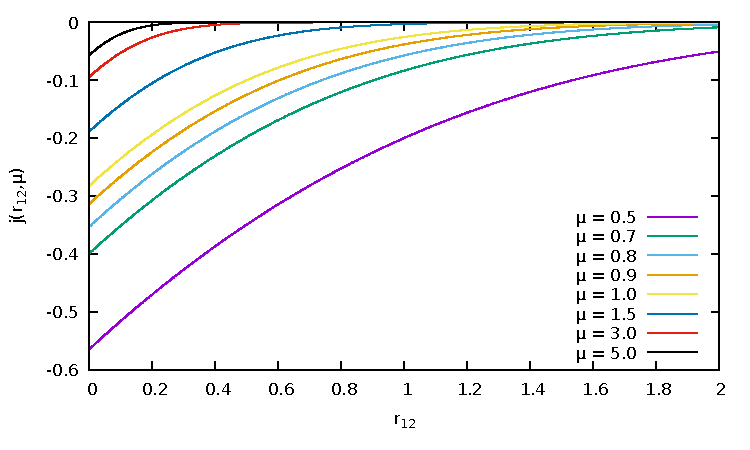
\includegraphics[width=0.45\linewidth]{small_mu_j.pdf}
%        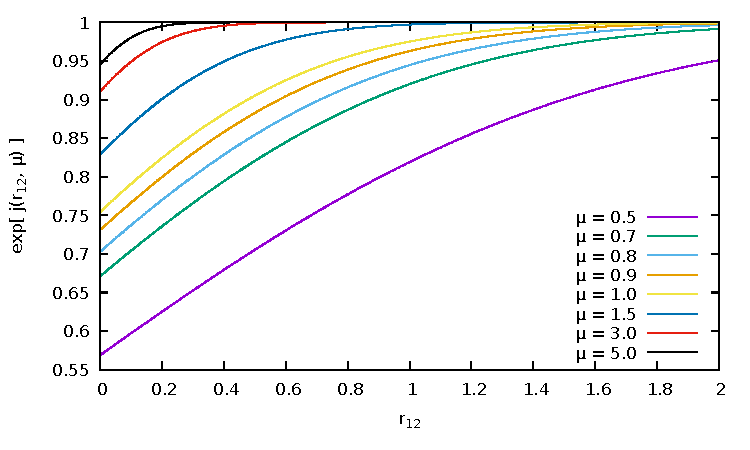
\includegraphics[width=0.45\linewidth]{small_mu_exp_j.pdf}\\
%        \caption{Shape of $u(r_{12};\mu)$ (up) and of $\mathcal{J}(r_{12};\mu) = \text{exp}\bigg(u(r_{12};\mu) \bigg) $ (bottom) for different values of $\mu$.}
%\end{figure*}
From Figure\ref{fig_j_mu}, one can see that: i) the larger the $\mu$, the more short-range is $u(r_{12};\mu)$, ii) the larger the $\mu$, the closer $u(r_{12};\mu)$ is from 0 and therefore the less impact the correlating factor has on the wave function, iii) the smaller the $\mu$, the deeper is the hole imposed by $\mathcal{J}(r_{12};\mu)$. 


\subsection{The general analytical form of  $\tilde{H}[\mu]$ and some of its properties}
\label{sec:ht_general}
\subsubsection{General form of $\tilde{H}[\mu]$ }
Having established the analytical expression of $u(r_{12};\mu)$, one can derive the general expression of the associated transcorrelated Hamiltonian.  
According to Eq. (2) of Ref. \onlinecite{CohLuoGutDobTewAla-JCP-19}, the similarity transformed Hamiltonian can be written as 
\begin{equation}
 \label{ht_def_g}
 e^{-\hat{\tau}} \hat{H} e^{\hat{\tau}} = H + \big[ H,\hat{\tau} \big] + \frac{1}{2}\bigg[ \big[H,\hat{\tau}\big],\hat{\tau}\bigg]
\end{equation}
where $\hat{\tau} = \sum_{i<j}u(\br{}_i,\br{}_j)$ and $\hat{H} = \sum_i -\frac{1}{2} \nabla^2_i + v(\br{}_i) + \sum_{i<j} \frac{1}{r_{ij}}$. 
This leads to the following similarity transformed Hamiltonian 
\begin{equation}
 \begin{aligned}
 \label{ht_def_gu}
 \tilde{H} & = H - \sum_i \bigg( \frac{1}{2} \nabla_i^2 \hat{\tau} + \big(\nabla_i \hat{\tau} \big) + \frac{1}{2} \big(\nabla_i \hat{\tau} \big)^2  \bigg) \\
           & = H - \sum_{i<j} \hat{K}(\bri{i},\bri{u}) - \sum_{i<j<k} \hat{L}(\bri{i},\bri{u},\bri{k}),
 \end{aligned}
\end{equation}
where the effective two- and three-body operators $\hat{K}(\bri{i},\bri{u})$ and $\hat{L}(\bri{i},\bri{u},\bri{k})$ are defined as
\begin{equation}
 \begin{aligned}
 \label{def_k}
  \hat{K}(\bri{1},\bri{2}) ) = \frac{1}{2} \bigg( &\nabla_1^2 u(\bri{1},\bri{2}) + \nabla_2^2u(\bri{1},\bri{2}) \\
                                               + &\big(\nabla_1 u(\bri{1},\bri{2}) \big) ^2 + \big(\nabla_1 u(\bri{1},\bri{2}) \big) ^2 \bigg) \\
                                               + &\nabla_1 u(\bri{1},\bri{2}) \cdot \nabla_2 + \nabla_2 u(\bri{1},\bri{2}) \cdot \nabla_1,
 \end{aligned}
\end{equation}
\begin{equation}
 \begin{aligned}
 \label{def_k}
  \hat{L}(\bri{1},\bri{2},\bri{3}) ) = & \nabla_1 u(\bri{1},\bri{2}) \cdot \nabla_1 u(\bri{1},\bri{3}) + \nabla_2 u(\bri{2},\bri{1}) \cdot \nabla_2 u(\bri{2},\bri{3})  \\
                                     + & \nabla_3 u(\bri{3},\bri{1}) \cdot \nabla_3 u(\bri{3},\bri{2}).
 \end{aligned}
\end{equation}
Therefore, to obtain the analytical expression of the $\tilde{H}[\mu]$ for a general $N$-electron system, 
one needs to compute the actual form of the operators $\hat{K}(\bri{1},\bri{2})$ and $\hat{L}(\bri{1},\bri{2},\bri{3})$ when $u(\bri{1},\bri{2}) = u(r_{12},\mu)$. 

\subsection{Analytical form for the operators $\hat{K}(\bri{1},\bri{2}) $ and $\hat{L}(\bri{1},\bri{2},\bri{3})$ }
To compute the operators $\hat{K}(\bri{1},\bri{2})$ and $\hat{L}(\bri{1},\bri{2},\bri{3}) $ one needs to compute first the gradient of $u(r_{12},\mu)$ with respect to $\bri{1}$ which reads 
\begin{equation}
 \label{eq:nabla_u}
 \begin{aligned}
 \nabla_1 u(\br{}_1,\br{}_2) = \frac{1 - \text{erf}(\mu r_{12})}{2 r_{12}} \big( \br{}_1 - \br{}_2 \big).
 \end{aligned}
\end{equation}
Then, the term $\big(\nabla_1 u(\bri{1},\bri{2}) \big) ^2 + \big(\nabla_1 u(\bri{1},\bri{2}) \big) ^2$ is simply 
\begin{equation}
 \begin{aligned}
 \big(\nabla_1 u(\bri{1},\bri{2}) \big) ^2 + \big(\nabla_2 u(\bri{1},\bri{2}) \big) ^2 = \frac{\bigg(1 - \text{erf}(\mu r_{12}) \bigg)^2}{2}.
 \end{aligned}
\end{equation}
Then, the non hermitian operators in $\hat{K}(\bri{1},\bri{2})$ contains 
\begin{equation}
 \begin{aligned}
 \nabla_1 u(\br{}_1,\br{}_2) \cdot \nabla_1  = &\frac{1 - \text{erf}(\mu r_{12})}{2 r_{12}} \\ 
                                          &\bigg( (x_1 - x_2) \deriv{}{x_1}{} + (y_1 - y_2) \deriv{}{y_1}{} + (z_1 - z_2) \deriv{}{z_1}{}\bigg),
 \end{aligned}
\end{equation}
and as $\nabla_1 u(\br{}_1,\br{}_2) = - \nabla_2 u(\br{}_1,\br{}_2)$,   
the total non hermitian operator in $\hat{K}(\bri{1},\bri{2})$ can be written as 
\begin{equation}
 \begin{aligned}
 \label{def_non_hermit}
& \nabla_1 u(\br{}_1,\br{}_2) \cdot \nabla_1 + \nabla_2 u(\br{}_1,\br{}_2) \cdot \nabla_2 = \frac{1 - \text{erf}(\mu r_{12})}{2 r_{12}} \\
& \bigg( (x_1 - x_2) \big( \deriv{}{x_1}{} - \deriv{}{x_2}{} \big) +
         (y_1 - y_2) \big( \deriv{}{y_1}{} - \deriv{}{y_2}{} \big)  \\
&  +      (z_1 - z_2) \big( \deriv{}{z_1}{} - \deriv{}{z_2}{} \big)\bigg).
 \end{aligned}
\end{equation}
One can notice that the form of Eq. \eqref{def_non_hermit} provides an explicit form to compute analytical integrals with Gaussian types functions. 
Nevertheless, one can notice that as 
\begin{equation}
 \deriv{}{r_{12}^x}{} = \frac{1}{2} \bigg( \deriv{}{x_1}{} - \deriv{}{x_2}{} \bigg),
\end{equation}
one can write 
\begin{equation}
 \begin{aligned}
 \label{eq:nabla_i_nabla0}
& \nabla_1 u(\br{}_1,\br{}_2) \cdot \nabla_1 + \nabla_2 u(\br{}_1,\br{}_2) \cdot \nabla_2 = \frac{1 - \text{erf}(\mu r_{12})}{r_{12}} \big( \br{}_1 - \br{}_2 \big) \cdot \nabla_{\br{}_{12}}.
 \end{aligned}
\end{equation}
Then, introducing the spherical coordinate system for $\br{}_1 - \br{}_2$ in terms of ${\bf e}_u= \frac{\br{}_1 - \br{}_2}{r_{12}}$ and the angle $\theta$ and $\phi$, one can write 
\begin{equation}
 \nabla_{\br{}_{12}} = \deriv{}{r_{12}}{} {\bf e}_u + \frac{1}{r_{12}} \deriv{}{\theta}{} {\bf e}_{\theta} + \frac{1}{r_{12} \sin(\theta)} \deriv{}{\phi}{} {\bf e}_\phi,
\end{equation}
and as $\br{}_1 - \br{}_2 = r_{12} {\bf e}_u$ one obtains
\begin{equation}
 \big( \br{}_1 - \br{}_2 \big) \cdot \nabla_{\br{}_{12}} = r_{12} \deriv{}{r_{12}}{},
\end{equation}
and therefore 
\begin{equation}
 \begin{aligned}
 \label{eq:nabla_i_nabla1}
 \nabla_1 u(\br{}_1,\br{}_2) \cdot \nabla_1 + \nabla_2 u(\br{}_1,\br{}_2) \cdot \nabla_2 = \bigg( 1 - \text{erf}(\mu r_{12})\bigg) \deriv{}{r_{12}}{},
 \end{aligned}
\end{equation}
which is a more compact expression than Eq.\eqref{def_non_hermit}

The computation of the Laplacian is a little more tedious, but after some derivations it comes  
\begin{equation}
 \begin{aligned}
 \label{eq:d2_x1_2}
 &\nabla_1^2 u(\bri{1},\bri{2}) + \nabla_2^2u(\bri{1},\bri{2})\\ 
 & = 2 \times \bigg( \frac{1 - \text{erf}(\mu r_{12})}{r_{12}} - \frac{\mu}{\sqrt{\pi}} e^{-\big(\mu r_{12} \big)^2}  \bigg).
 \end{aligned}
\end{equation}

Summing all terms to recombine $\hat{K}(\bri{1},\bri{2})$ reads 
\begin{equation}
 \label{eq:k_final}
  \begin{aligned}
   \hat{K}(\bri{1},\bri{2}) = & \frac{1 - \text{erf}(\mu r_{12})}{r_{12}} - \frac{\mu}{\sqrt{\pi}} e^{-\big(\mu r_{12} \big)^2} + \frac{\bigg(1 -     \text{erf}(\mu r_{12}) \bigg)^2}{4} \\
& - \bigg( \text{erf}(\mu r_{12}) - 1\bigg) \deriv{}{r_{12}}{}.
  \end{aligned}
\end{equation}
Similarly, the computation of $\hat{L}(\bri{1},\bri{2},\bri{3}) $ 
\begin{equation}
 \label{eq:l_final}
 \begin{aligned}
 \hat{L}_\mu(\bri{1},\bri{2},\bri{3}) = & \frac{1 - \text{erf}(\mu r_{12})}{2 r_{12}} \bri{12} \cdot \frac{1 - \text{erf}(\mu r_{13})}{2 r_{13}} \bri{13} \\
                                      + & \frac{1 - \text{erf}(\mu r_{12})}{2 r_{12}} \bri{21} \cdot \frac{1 - \text{erf}(\mu r_{23})}{2 r_{23}} \bri{23} \\
                                      + & \frac{1 - \text{erf}(\mu r_{13})}{2 r_{13}} \bri{31} \cdot \frac{1 - \text{erf}(\mu r_{32})}{2 r_{32}} \bri{32}.
 \end{aligned}                    
\end{equation}

\subsection{Analytical form of $\tilde{H}[\mu]$}
Having established the explicit form of $\hat{K}(\bri{1},\bri{2})$ and $\hat{L}_\mu(\bri{1},\bri{2},\bri{3})$, one can now 
look at the explicit analytical form of the transcorrelated Hamiltonian $\tilde{H}[\mu]$ obtained with $u(r_{12};\mu)$,  
which, by injecting the form of Eqs. \eqref{eq:k_final} and \eqref{eq:l_final} in Eq.\eqref{ht_def_gu}, which gives
\begin{equation}
  \begin{aligned}
 \label{eq:exp_ht_mu}
   \tilde{H}[\mu] = & h_c + \sum_{i<j} \bigg( \tilde{\mathcal{W}}_{ee}(r_{ij},\mu) + \tilde{t}[\mu] \bigg) - \sum_{i<j<k} \hat{L}_\mu(\bri{1},\bri{2},\bri{3})
  \end{aligned}
\end{equation}
where $ \tilde{\mathcal{W}}_{ee}(r_{ij},\mu)$ is the scalar effective two-body potential of  $\tilde{H}[\mu]$
\begin{equation}
 \begin{aligned}
 \tilde{\mathcal{W}}_{ee}(r_{ij},\mu)  =  \frac{\text{erf}(\mu r_{ij})}{r_{ij}} + \frac{\mu}{\sqrt{\pi}} e^{-\big(\mu r_{ij} \big)^2} - \frac{\bigg(1 -     \text{erf}(\mu r_{ij}) \bigg)^2}{4}, 
 \end{aligned}
\end{equation}
and $\tilde{t}[\mu]$ is a non hermitian two-body differential operator 
\begin{equation}
 \begin{aligned}
 \tilde{t}[\mu] =  \bigg( \text{erf}(\mu r_{ij}) - 1\bigg) \deriv{}{r_{ij}}{}.
 \end{aligned}
\end{equation}

In order to have a pictorial representation of $ \tilde{\mathcal{W}}_{ee}(r_{ij},\mu)$, we illustrate in Fig\ref{fig_wee_mu} its shape for different values of $\mu$. 
%\begin{figure*}
% \label{fig_wee_mu}
%        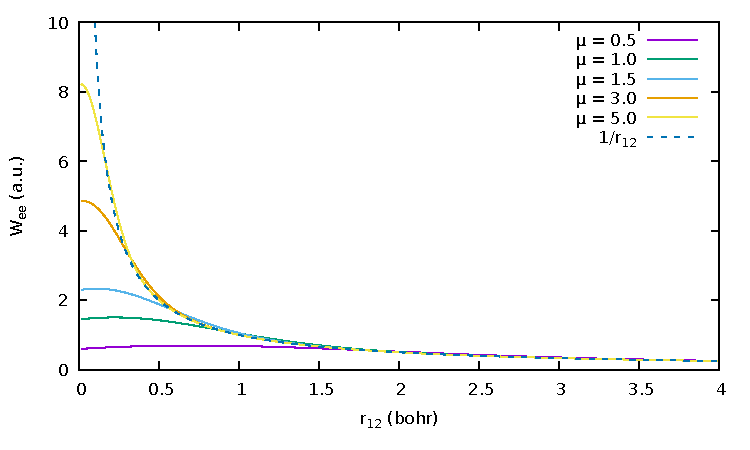
\includegraphics[width=0.45\linewidth]{w_ee.pdf}
%        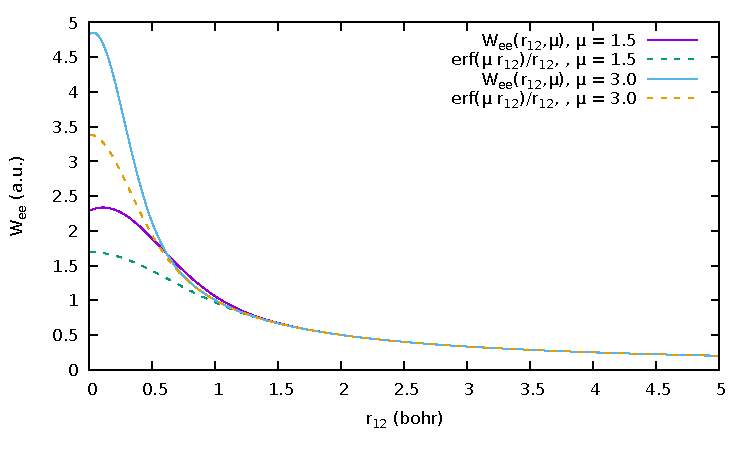
\includegraphics[width=0.45\linewidth]{w_ee_bis.pdf}\\
%        \caption{Shape of $\tilde{\mathcal{W}}_{ee}(r_{12},\mu)$ (up) and comparison with $\frac{\text{erf}(\mu r_{12}}{r_{12}}$ (bottom) for different values of $\mu$.}
%\end{figure*}
From  Fig.\ref{fig_wee_mu} we can see that the scalar effective potential $ \tilde{\mathcal{W}}_{ee}(r_{ij},\mu)$ 
is non divergent, increases when $\mu$ increases and globally resembles the long-range interaction used in RS-DFT at large $r_{12}$. 
Nevertheless, as observed from Fig.\ref{fig_wee_mu}, it is significantly different 
from the long-range interaction at small $r_{12}$, 
and it is not monotonic and attractive (\textit{i.e.} $\lim_{r_{12} \rightarrow 0} \deriv{}{r_{12}}{} \tilde{\mathcal{W}}_{ee}(r_{ij},\mu) >0 $). 
This difference with respect to the long-range interaction can be understood as the equation obtained to derive the Jastrow factor only takes into account the first-order derivative of $u(r_{12},\mu)$ (see Eqs.\eqref{def_j_00} and \eqref{def_j_0}). 
If one desires to impose that $\tilde{\mathcal{W}}_{ee}(r_{12},\mu) = \frac{\text{erf}(\mu r_{12})}{r_{12}}$, one would have to solve the non-linear differential equation 
\begin{equation}
 2 \deriv{u(r_{12})}{r_{12}}{} + r_{12} \bigg( \deriv{u(r_{12})}{r_{12}}{2} + \bigg[ \deriv{u(r_{12})}{r_{12}}{} \bigg]^2\bigg) = 1 - \text{erf}(\mu r_{12}), 
\end{equation}
whose solution is unknown to the best of the author knowledge. 
\subsection{Variation of $\tilde{H}[\mu]$ with $\mu$}
\label{sec:h_mu_lim}
Regarding now the variation of $\tilde{H}[\mu]$, one expects that as 
\begin{equation}
 \label{eq:lim_mu_0}
 \lim_{\mu  \rightarrow \infty }u(\mu,r_{12}) = 0, 
\end{equation}
one recovers the usual Hamiltonian in the ${\mu  \rightarrow \infty }$ limit:
\begin{equation}
 \label{eq:lim_mu_1}
 \lim_{\mu \rightarrow \infty} \tilde{H}[\mu] = H.
\end{equation}
Nevertheless, in the large $\mu$ limit, one can notice that 
\begin{equation}
 \label{eq:lim_mu_3}
 \lim_{\mu \rightarrow \infty} \tilde{\mathcal{W}}_{ee}(r_{12})  = \frac{1}{r_{12}} + \delta(r_{12}) 
\end{equation}
where $\delta(r_{12})$ is the Dirac distribution, and as the firs-order differential term vanishes in the large $\mu$ limit (see Eq.\eqref{eq:exp_ht_mu}), one could be tempted to write that 
\begin{equation}
 \begin{aligned}
 \label{eq:lim_mu_4}
 \lim_{\mu \rightarrow \infty} \tilde{H}[\mu]& = h_c + \frac{1}{r_{12}} + \delta(r_{12}) \\
                                             & = H + \delta(r_{12})  \\
                                             & \ne H,
 \end{aligned}
\end{equation}
which seems to contradict the intuitive limit of Eq.\eqref{eq:lim_mu_1}. 

Nevertheless, as the right hand side of Eq.\eqref{eq:lim_mu_4} contains a Delta distribution, it must be considered in the sense of distributions an not point wise. 
Therefore, considering a generic bounded square integrable wave function $\psi(\br{}_1,\hdots,\br{}_N)$ yielding to a integrable pair density $n_2(\br{}_1,\br{}_2)$, the equality between $\tilde{H}[\mu]$ and $H$ is, in the sense of distributions, defined by the following equality 
\begin{equation}
 \label{eq:lim_mu_5}
 \begin{aligned}
& \matelem{\psi}{H}{\psi} = \lim_{\mu \rightarrow \infty} \matelem{\psi}{\tilde{H}[\mu]}{\psi} \\
& \Leftrightarrow H = \tilde{H}[\mu],
 \end{aligned}
\end{equation}
and considering the limit for of $\tilde{H}[\mu]$ (see Eq.\eqref{eq:lim_mu_4}), it implies that 
\begin{equation}
 \label{eq:lim_mu_6}
 \int \text{d}\br{}_1 \text{d}\br{}_2 n_2(\br{}_1,\br{}_2) \delta(r_{12}) = 0.
\end{equation}
To intuitively show Eq.\eqref{eq:lim_mu_6}, one can perform a series of change of variable $(\br{}_1,\br{}_2)\rightarrow (\br{}_{12},\frac{1}{2}(\br{}_1 + \br{}_2))$ and then use the spherical coordinates for $\br{}_{12}$ 
\begin{equation}
 \int \text{d}\br{}_1 \text{d}\br{}_2 n_2(\br{}_1,\br{}_2) \delta(r_{12}) = \int \text{d}r{}_{12}  \tilde{n}_2(r_{12}) \delta(r_{12}) r_{12}^2 
\end{equation}
where $\tilde{n_2}(x)$ is the function $n_2(\br{}_1,\br{}_2)$ integrated over $(\br{}_1,\br{}_2)$ with the constraint that 
$|\br{}_1-\br{}_2| = x$. 
As the pair density $n_2(\br{}_1,\br{}_2)$ remains finite and is integrable, the function $\tilde{n}_2(x)$ 
cannot diverge faster than $\frac{1}{x}$ when $x\rightarrow 0$ and therefore one obtains that 
\begin{equation}
 \int \text{d}r{}_{12}  \tilde{n}_2(r_{12}) \delta(r_{12}) r_{12}^2 = 0,
\end{equation}
which implies Eq.\eqref{eq:lim_mu_1}. 

In the $\mu \rightarrow 0$ limit, the transcorrelated Hamiltonian $\tilde{H}[\mu]$ becomes simply 
\begin{equation}
 \label{eq:htilde_mu_low}
 \begin{aligned}
&\lim_{\mu \rightarrow 0} \tilde{H}[\mu] = h_c - \frac{1}{4} - \sum_{i<j}\deriv{}{r_{ij}}{} \\
 & - \frac{1}{4}\sum_{i<j<k}  \bigg(\frac{\bri{ij} }{ r_{ij}} \cdot \frac{\bri{ik} }{ r_{ik}} + \frac{\bri{ji} }{ r_{ji}} \cdot \frac{\bri{jk}  }{ r_{jk}} + \frac{\bri{ki} }{ r_{ki}} \cdot  \frac{\bri{kj} }{ r_{kj}} \bigg),
 \end{aligned}
\end{equation}
which means that all scalar electron-electron repulsive interaction have been replaced by a differential operator and a three electron interaction. 
It should be stressed that even if the $\mu \rightarrow 0$ limit of $\tilde{H}[\mu]$ is very unphysical, it conserves exactly the same spectrum than the usual Hamiltonian because it originates from a similarity transformation. 

At intermediate values of $\mu$, the scalar potential $\tilde{\mathcal{W}}_{ee}(r_{12},\mu) $ is non divergent, and can be repulsive or attractive at small $r_{12}$. One can therefore notice the diversity of physical content of $\tilde{H}[\mu]$ as a function of a unique parameter, $\mu$. 
Nevertheless, due to the property of the similarity transformation, in the limit of a complete basis set, the eigenvalues of $\tilde{H}[\mu]$, whatever the value of $\mu$ chosen, coincide with that of the physical Hamiltonian. An important point then is the convergence with respect to the basis set of the family of $\tilde{H}[\mu]$ for different values of $\mu$, which is tested for wide variety of two-electron systems in the next sections. 

\section{Detailed numerical study of $\tilde{H}[\mu]$ in the case of he He atom}
\label{sec:total_he}
The first part of our study concerns the convergence of the eigenvalues of $\tilde{H}[\mu]$ with respect to the basis set, and more precisely the dependence on $\mu$ of such convergence. 

Considering a given basis set $\basis$ and the corresponding projector $P_\basis$, one can define the transcorrelated Hamiltonian projected on $\basis$ by
\begin{equation}
 \tilde{H}[\mu]^{\basis} = P_\basis \tilde{H}[\mu] P_\basis,
\end{equation}
and its eigenvalues $E_i^{\basis}[\mu]$ and right eigenvectors $\phiimub$ satisfy 
\begin{equation}
 \tilde{H}[\mu]^{\basis} \ket{\phimub} = E_i^{\basis}[\mu] \ket{\phiimub}. 
\end{equation}
As long as the basis set $\basis$ is incomplete, because of its non hermitian nature, $\tilde{H}[\mu]^{\basis}$ looses the variational principle and therefore its eigenvalues have no reasons to be bounded from below.  

As pointed in section \ref{sec:h_mu_lim}, by varying $\mu$ one can go from a relatively usual repulsive Hamiltonian at large $\mu$ (even though it is non hermitian an non divergent), passing by an almost attractive Hamiltonian and even to a purely attractive Hamiltonian. 
As pointed in section \ref{sec:h_mu_lim}, even though $\tilde{H}[\mu]$ is still non hermitian as long as $\mu < \infty$, by varying $\mu$ one can change the nature of the electron-electron interaction in $\tilde{\mathcal{W}}_{ee}(r_{12},\mu)$ from a repulsive and non divergent interaction at large $\mu$ (an non divergent), passing by an almost attractive Hamiltonian and even to a purely attractive Hamiltonian. 
Considering such variation of $\tilde{H}[\mu]$ when varying $\mu$,  
its projection into a basis set $\tilde{H}[\mu]^{\basis}$ will behave differently as a function of $\mu$ 
and so will the right eigenvectors $\ket{\phiimub}$ and the corresponding eigenvalues $E_i^{\basis}[\mu]$. 
Therefore, we would like to study the behaviour of $\ket{\phiimub}$ and $E_i^{\basis}[\mu]$ as a function of both $\basis$ and $\mu$ to see whether the use of the new form of Jastrow factor $u(r_{12},\mu)$ can improve the convergence toward the exact energies  and eigenvectors. 
\subsection{$\mu$ dependence of the convergence of the ground state eigenvalue with respect to the basis set }
\subsubsection{Computational details}
We implemented all integrals needed for the computation of the matrix elements of $\tilde{H}[\mu]$ on a usual gaussian orbital basis set (see annexes for more details) together with the modification of the Slater rules due to the presence of the non hermitian term in $\tilde{H}[\mu]$. 
All implementation was done as a plugin of the program quantum package\cite{QP2}. 
We use the RHF molecular orbitals to build all matrix elements of $\tilde{H}[\mu]$, and then we solve the two-body problem giving full flexibility to $\phiimub$ (\textit{i.e.} $\phiimub$ is expressed as a linear combination of all possible Slater determinants within a given basis set $\basis$) with a non hermitian eigensolver to obtain both right and left eigenvectors. 
%The study was performed using the augmented Dunning basis aug-cc-pVXZ (X=D,T,Q,5), hereafter referred as AVXZ. 

\subsubsection{Numerical results: ground state energies}
\label{sec:total_e}
We report in Table \ref{table_conv_e_mu} the ground state eigenvalue $E_i^{\basis}[\mu]$ of $\tilde{H}[\mu]^{\basis}$ in the AVXZ basis sets (X=D,T,Q,5) for different values of $\mu$, and we report in Figure \ref{fig_conv_e_mu} the graphical representation of such data. 
Several observations can be done from these data. First, because of the loose of the variational principle, $E_0^{\mu}$ can take values below the exact non relativistic energy, and the smaller the $\mu$, the more pronounced is such effect. 
Nevertheless, one can also observe that, for each $\mu$, the error with respect to the exact energy gets smaller  
when enlarging the basis set. Also, qualitatively, one can observe that there are two regimes of $\mu$: $\mu \in[0.05,0.7]$ where the $E_0^\mu$ is always below $E_0$ and $\mu\ge 0.7$ where $E_0^\mu$ converges from above, as if the variational principle still applied. 
As $\mu$ increases, the difference between $E_0^\mu$ and $E_0^\text{FCI}$ in a given basis set diminishes, 
which is expected as in the $\mu \rightarrow \infty$ limit, one obtains that  $\tilde{H}[\mu] \rightarrow H$. 

Coming now to the speed of convergence of $E_0^\mu$ with respect to the basis set, it is always faster than that of $E_0^\text{FCI}$ as long as $\mu \ge 0.2$. 
To quantify better such observations, one can identify the basis set from which the error with respect to the exact non relativistic energy is smaller, in absolute value, than 1mH. 
For $0.3\ge\mu\ge0.4$ one can see that the error with respect to $E_0$ is never larger, in absolute value, than 1mH whatever the basis set used, which represents a strong improvement with respect to the FCI. For $0.5\ge \mu \ge 1.0$ the 1mH error threshold is reached at the aug-cc-pVTZ level and the accuracy are comparable to the FCI in the aug-cc-pV5Z basis set. For $1.6\ge \mu \ge 3.0$, such accuracy is reached at the aug-cc-pVQZ level, whenever such accuracy is reached at the aug-cc-pV5Z level using the regular FCI Hamiltonian. 
Therefore one can conclude that the use of a simple Jastrow factor such as $u(r_{12};\mu)$ within the transcorrelated framework can strongly improve the speed of convergence of the total energy of the helium atom with a quite wide range of values of $\mu$ ranging from $\mu=0.2$ to $\mu=1.6$. 
%\begin{figure*}
% \label{fig_conv_e_mu}
%        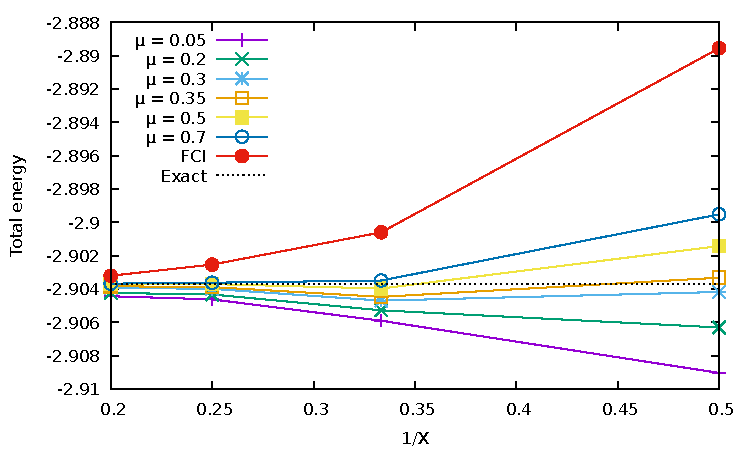
\includegraphics[width=0.45\linewidth]{E_conv_basis_small_mu.pdf}
%        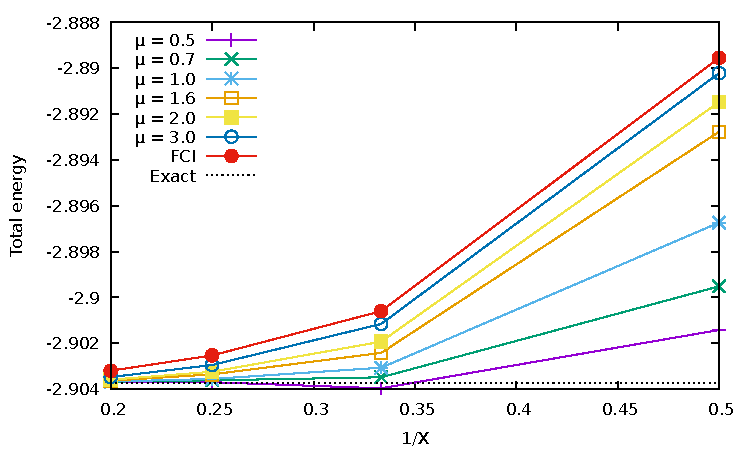
\includegraphics[width=0.45\linewidth]{E_conv_basis_large_mu.pdf}\\
%        \caption{Convergence of the ground state eigenvalue of $\tilde{H}[\mu]$ with respect to the AVXZ basis set series (X=D,T,Q,5) for different values of $\mu$.}
%\end{figure*}

\begin{table*}
\label{table_conv_e_mu}
\caption{Ground state eigenvalue (in Hartree) of $\tilde{H}[\mu]$ for the He atom with the AVXZ (X=D,T,Q,5) basis sets for different values of $\mu$, and error (in mH) with respect to the exact non relativistic energy.}
\begin{ruledtabular}
\begin{tabular}{llllllllllll}
 Basis/$\mu$&0.05                 & 0.2                   & 0.3                   & 0.35                  & 0.5                  & 0.7                   \\
\hline
 AVDZ       &  -2.909031 (-5.31)  &    -2.906309 (-2.58)  &    -2.904172 (-0.45)  &    -2.903317 (0.41)   &    -2.901420 (2.3)   &    -2.899516 (4.21)   \\
 AVTZ       &  -2.905898 (-2.17)  &    -2.905278 (-1.55)  &    -2.904691 (-0.97)  &    -2.904468 (-0.74)  &    -2.903969 (-0.24) &    -2.903488 (0.24)   \\
 AVQZ       &  -2.904621 (-0.9)   &    -2.904325 (-0.6)   &    -2.903986 (-0.26)  &    -2.903879 (-0.15)  &    -2.903702 (0.02)  &    -2.903620 (0.1)     \\
 AV5Z       &  -2.904428 (-0.7)   &    -2.904229 (-0.51)  &    -2.903928 (-0.2)   &    -2.903834 (-0.11)  &    -2.903702 (0.02)  &    -2.903676 (0.05)   \\
\hline
 Basis/$\mu$ & 1.0                  & 1.6                  & 2.0                  & 3.0                  & $\infty$ (FCI)        & Exact NR              \\
\hline
 AVDZ        &    -2.896734 (6.99)  &    -2.892773 (10.95) &    -2.891477 (12.25) &    -2.890212 (13.51) &    -2.889548 (14.18)  & -2.903724             \\
 AVTZ        &    -2.903069 (0.66)  &    -2.902421 (1.3)   &    -2.901932 (1.79)  &    -2.901159 (2.56)  &    -2.900598 (3.13)   &                       \\
 AVQZ        &    -2.903558 (0.17)  &    -2.903359 (0.36)  &    -2.903244 (0.48)  &    -2.902951 (0.77)  &    -2.902534 (1.19)   &                       \\
 AV5Z        &    -2.903675 (0.05)  &    -2.903634 (0.09)  &    -2.903592 (0.13)  &    -2.903479 (0.24)  &    -2.903201 (0.52)   &                       \\
\end{tabular}
\end{ruledtabular}
\end{table*}

\subsection{Study of the ground state eigenvector in real space}
In Sec.\ref{sec:total_e} we shown the improvement of the speed of convergence of the ground state energies $E_i^{\basis}[\mu]$ of the helium atom, which was effective for a quite large range of $\mu$ starting from $\mu=0.2$ to $\mu=3.0$. 
Nevertheless, one can wonder if this good behavior results from a kind of error cancellation or if there is indeed a deeper mathematical reason for such an improvement of speed of convergence. 
To answer that question, we investigate some properties of the ground state eigenvectors of different types of Hamiltonians in real space. 

Theoretically if, for a given value of $\mu$, $\tilde{H}[\mu]$ is perfectly well represented in a given basis set $\mathcal{B}$ (\textit{i.e.} $\tilde{H}[\mu]^{\basis} = \tilde{H}[\mu]$), then all its eigenvalues coincide with that of the exact Hamiltonian (\textit{i.e.} developed in a complete basis set). If one focusses now on the exact ground state eigenvector $\phimu$ of $\tilde{H}[\mu]$, it is directly related to the exact ground state wave function $\psiex$ by the Jastrow factor $u(r_{12},\mu)$ through 
\begin{equation}
 \psiex(\br{}_1,\br{}_2) =  \frac{1}{\sqrt{\mathcal{N}^{\mu}}} e^{u(r_{12},\mu)} \phimu(\br{}_1,\br{}_2), 
\end{equation}
where the normalization factor $\mathcal{N}^{\mu}$ is simply 
\begin{equation}
  \mathcal{N}^{\mu} = \matelem{\phimu}{e^{2 u(r_{12},\mu)}}{\phimu}.
\end{equation}
Therefore, in a given basis set $\basis$, the right eigenvector $\phimub$ of $\tilde{H}[\mu]^{\basis}$ can be used to estimate the exact ground state wave function $\psiex$ through 
\begin{equation}
 \psimub(\br{}_1,\br{}_2) = \frac{1}{\sqrt{\mathcal{N}_{\basis}^{\mu}}}e^{u(r_{12},\mu)}\phimub(\br{}_1,\br{}_2),
\end{equation}
where the normalization factor $\mathcal{N}_{\basis}^{\mu}$ is simply
\begin{equation}
  \mathcal{N}_{\basis}^{\mu} = \matelem{\phimub}{e^{2 u(r_{12},\mu)}}{\phimub}.
\end{equation}
Then, the quality of a given basis set $\basis$ for a given $\mu$ can be also quantified from the vicinity between $\psimub(\br{}_1,\br{}_2)$ and the exact wave function $\psiex(\br{}_1,\br{}_2)$, in the $L^2$ sense for instance. 
For this study, we approximate the exact ground state wave function $\psiex(\br{}_1,\br{}_2)$ of the helium atom by the wave function developed by Umrigar \textit{et. al.}\cite{UmrGon-PRA-94} which contains explicitly the $r_{12}$ coordinate and which provides a total energy accurate up to twelve digits.  
We plotted a cutting of $\psiex(\br{}_1,\br{}_2)$ and  $\psimub(\br{}_1,\br{}_2) $ with different basis sets and values of $\mu$. The cutting used is the following: we set two electrons on a circle of radius $r=0.5$ a.u. from the nucleus and look at the wave functions as a function of the angle $\theta_{12}$ between the $\bri{1}$ and $\bri{2}$. 

We report in Figs \ref{fig:mu_0.3_dz_3} and \ref{fig:mu_1.0_dz_3} the plot of the right eigenvector $\phimub(\br{}_1,\br{}_2)$, estimated exact wave function $\psimub(\br{}_1,\br{}_2)$ for $\mu=0.3$ and $\mu=1.0$ (respectively) and compared to the exact wave function $\psiex(\br{}_1,\br{}_2)$ and FCI wave function for $r=0.5\,a.u.$. 
%\begin{figure*}
% \label{fig:mu_0.3_dz_3}
%        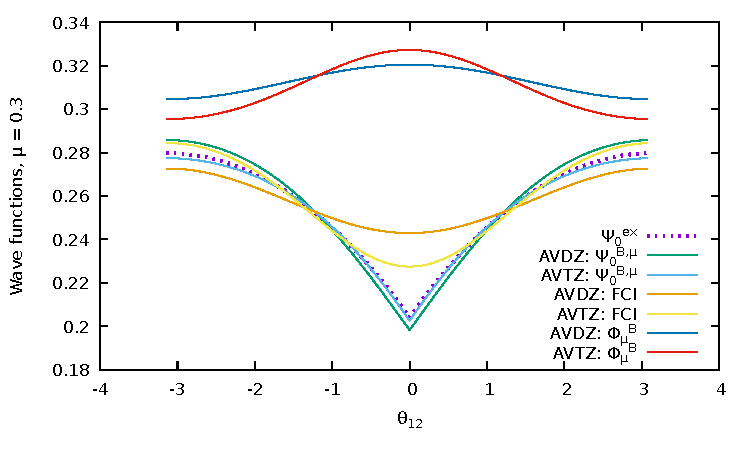
\includegraphics[width=0.45\linewidth]{plots/He//He_mu_0_3_cusp_avdz_avtz_3.pdf}
%        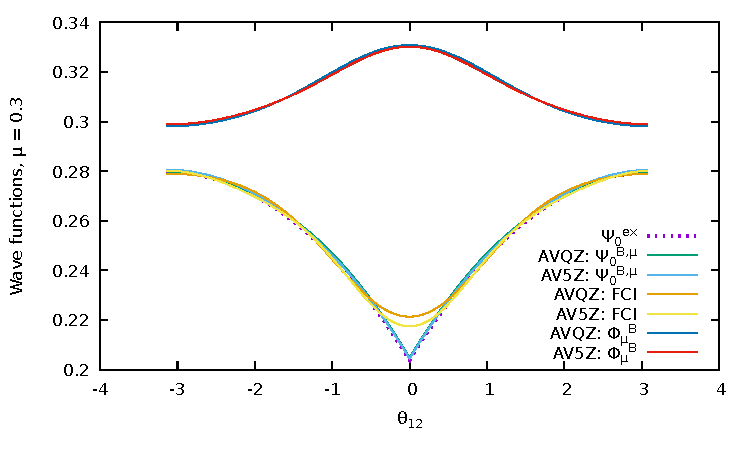
\includegraphics[width=0.45\linewidth]{plots/He/He_mu_0_3_cusp_avqz_av5z_3.pdf}\\
%        \caption{
%        Helium atom, radius $r=0.5$ a.u.: approximation of the exact wave function $\psimub(\br{}_1,\br{}_2)$ and right eigenvector $\phimub(\br{}_1,\br{}_2)$ for $\mu=0.3$ in the AVDZ and AVTZ basis sets (left) and AVQZ and AV5Z (right). Comparison with the FCI wave function in the same basis sets and the estimated exact wave function $\psiex(\br{}_1,\br{}_2)$.  }
%\end{figure*}

%\begin{figure*}
% \label{fig:mu_1.0_dz_3}
%        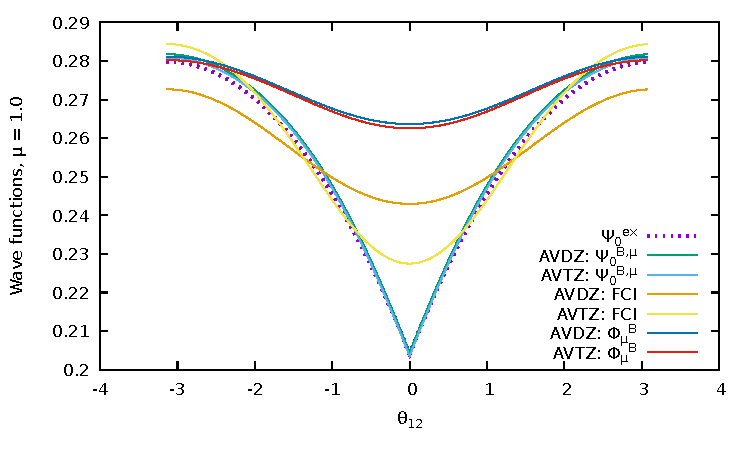
\includegraphics[width=0.45\linewidth]{plots/He/He_mu_1_0_cusp_avdz_avtz_3.pdf}
%        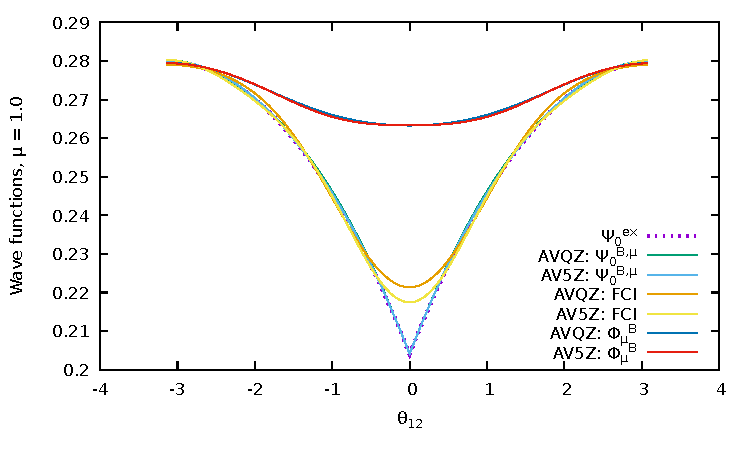
\includegraphics[width=0.45\linewidth]{plots/He/He_mu_1_0_cusp_avqz_av5z_3.pdf}\\
%        \caption{
%        Helium atom, radius $r=0.5$ a.u.: approximation of the exact wave function $\psimub(\br{}_1,\br{}_2)$ and right eigenvector $\phimub(\br{}_1,\br{}_2)$ for $\mu=1.0$ in the AVDZ and AVTZ basis sets (left) and AVQZ and AV5Z (right). Comparison with the FCI wave function in the same basis sets and the estimated exact wave function $\psiex(\br{}_1,\br{}_2)$.  }
%\end{figure*}


From these figure, one can notice that: 
i) the right eigenvector $\phimub(\br{}_1,\br{}_2)$ converges faster than the FCI wave function with respect to the basis set, 
ii) that for $\mu=0.3$ the wave function $\phimub(\br{}_1,\br{}_2)$ presents a maximum at $r_{12}=0$, whereas for $\mu=1.0$ it has a minimum at coalescence just as the FCI wave function, 
iii) the wave function $\phimub(\br{}_1,\br{}_2)$ is always larger that the FCI one when $r_{12}\approx 0$. 
iv) that $\psimub(\br{}_1,\br{}_2)$ provides a remarkably good approximation to $\psiex(\br{}_1,\br{}_2)$ from the AVTZ basis set, 

The understanding of such observations can be provided by the mathematical and physical investigation of the construction of $\tilde{H}[\mu]$. 

i) The shape of the Jastrow factor $u(r_{12};\mu)$ leading to the transcorrelated Hamiltonian is such that as long as $\mu < \infty$, the effective potential $\tilde{\mathcal{W}}_{ee}(r_{12},\mu)$ in $\tilde{H}[\mu]$ is non divergent, and therefore its eigenfunctions do not have to fulfill the cusp condition which leads to a faster convergence with $\basis$. 
Nevertheless, one can also remark that for $\mu > 0.5$, the speed of convergence deteriorates as $\mu$ increases, even though it remains finite. This can be explained by the fact that even if $\tilde{\mathcal{W}}_{ee}(r_{12},\mu)$ remains bounded from above, when $\mu$ is large such operator is poorly represented in a finite basis set. 

ii) The fact that the wave function $\phimub(\br{}_1,\br{}_2)$ presents a maximum at $r_{12}=0$ for $\mu=0.3$ whereas it provides a minimum for $\mu=1.0$ or the FCI wave function can be explained by the shape of the effective potential $\tilde{\mathcal{W}}_{ee}(r_{12},\mu)$: the latter is much more attractive when $r_{12}\approx 0$ for $\mu=0.3$ than for $\mu = 1.0$ (see Fig \ref{fig_wee_compare} for a graphical representation). 

iii) Similarly, as for any $\mu < \infty$ one has that $\tilde{\mathcal{W}}_{ee}(r_{12},\mu) <\frac{1}{r_{12}}$, the value of the eigenvector of $\phimub(\br{}_1,\br{}_2)$ is necessary larger than the FCI wave function at $r_{12}=0$ as in the latter the interaction is more repulsive. This implies that the on-top pair density (\textit{i.e.} the probability of finding two electrons at the same position) is necessary larger for the eigenvectors of $\tilde{H}[\mu]$ than that for the eigenvectors of $H$.

iv) The fact that $\psimub(\br{}_1,\br{}_2)$ provides  such a good approximation of $\psiex(\br{}_1,\br{}_2)$ in real space can be investigate through the prism of the local energy. 
The local energy $E_{\text{loc}}[\psi](\br{}_1,\br{}_2)$ associated to a given wave function $\psi$ is defined as 
\begin{equation}
 E_{\text{loc}}[\psi](\br{}_1,\br{}_2) = \frac{H\psi(\br{}_1,\br{}_2)}{\psi(\br{}_1,\br{}_2)},
\end{equation}
and is such that 
\begin{equation}
 \int \text{d}\br{}_1\,\,\text{d}\br{}_2\,\, E_{\text{loc}}[\psi](\br{}_1,\br{}_2) \big|\psi(\br{}_1,\br{}_2)\big|^2= \matelem{\psi}{H}{\psi}.
\end{equation}
Therefore, one can 
%\begin{figure*}
% \label{fig_wee_compare}
%        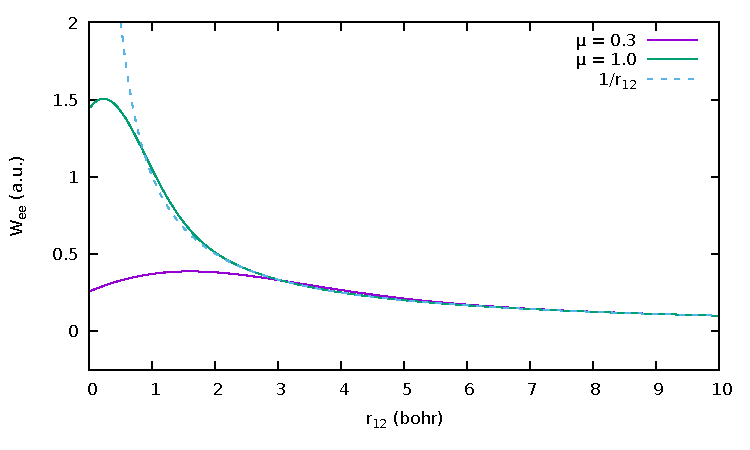
\includegraphics[width=1.00\linewidth]{w_ee_compare.pdf}
%        \caption{
%        Effective potential $\tilde{\mathcal{W}}_{ee}(r_{12},\mu)$ for $\mu=0.3$ and $\mu=1.0$, compared to the usual $1/r_{12}$ Coulomb interaction.}
%\end{figure*}

\section{Study of the helium isoelectronic series}
\label{sec:iso_elec}
Having investigated in the case of the helium atom the behaviour of both the eigenvalues and eigenvectors of $\tilde{H}[\mu]$ with both $\mu$ and the basis set used, we now study the ground state energies of the isoelectronic series of the helium atom H$^{-}$ to Ne$^{8+}$. As seen from the previous study on the helium atom, the quality of the eigenvalues of $\tilde{H}[\mu]$ depends on the value of $\mu$ but there is a quite wide regimes of $\mu$ for which they converge significantly faster with the basis set with respect to the usual Hamiltonian. Of course, the 'optimal' range of $\mu$ might depend on the system and we investigate here different approaches to systematically find a reasonable value of $\mu$ and test it on this isoelectronic series which consist in weakly correlated covering a quite wide range of densities. 
As in the study of the helium atom of Sec \ref{sec:total_h}, in a given basis set $\basis$ and for a given system, we use RHF molecular orbitals and the full flexibility is given to the eigenvectors $\ket{\phimub}$. 

In order to find a systematic way to determine a reasonable value of $\mu$, one must keep in mind the physical meaning of such quantity: it has the unit of an inverse distance, and determines, at leading order, the depth of the hole imposed by the Jastrow factor. 
Therefore, it must have the typical scale of the inverse of correlation effects, which of course strongly depends on the system through its density for instance. In the context of RS-DFT, Toulouse \textit{et. al.}\cite{TouColSav-JCP-05} have investigated different flavour of $\mu$ varying in space through the density of the system in a given point in space. 
More specifically, they introduced (see Eq. (12) of \onlinecite{TouColSav-JCP-05}) a range separation parameter typical for correlation effects in the uniform electron gas (UEG) 
\begin{equation}
 \mursc({\bf r}) =  \frac{2\sqrt{\alpha / \pi}}{\sqrt{r_s({\bf r})}},
\end{equation}
with $\alpha = (9 \pi/4)^{-1/3}$ and $r_s = (4 \pi n/3)^{-1/3}$. 
Such function $\mursc({\bf r})$ depends on the system and on the position in space through the density $n({\bf r})$ of the system at a given point ${\bf r}$. 
Therefore, we propose here to use the average value of $\mursc({\bf r})$ over the Hartree Fock electronic density to define the value of $\mu$ for a specific system in a given basis set:
\begin{equation}
 \label{eq:mu_av_rsc}
 \murscav = \frac{1}{N_e}\int \text{d}{\bf r} \mursc({\bf r}) n_{\text{HF}}({\bf r}) 
\end{equation}
where $n_{\text{HF}}({\bf r})$ is the HF density and $N_e$ the number of electrons in the system. 
We report in Table \ref{table_conv_e_mu_iso} the convergence with respect to the basis set $\basis$ the error with respect to the exact ground state energies of the isoelectronic series of the helium atom using $\murscav$ as value of $\mu$ in $\tilde{H}[\mu]$. 
We also report in the column $\muav$ of the Table \ref{table_conv_e_mu_iso} the value of $\murscav$ in the double-zeta quality basis for each system, the value in larger basis sets vary by less than $0.1\%$. 
As one can observe from  Table \ref{table_conv_e_mu_iso}, the ground state energies of $\tilde{H}[\murscav]$ converge much faster than that of the usual Hamiltonian as the MAD for the ground state energies is of 2.64 mH, 0.48 mH and 0.26 mH in the double-, triple- and quadruple zeta quality basis sets (respectively) whereas it is of 12.16 mH, 4.71 mH and 1.64 mH for the usual Hamiltonian. Also, one can observe that, except for the low density systems such as the H${^-}$ and He species, it converges from below the exact ground state energy. Regarding now the value of $\murscav $, one can notice that it increases with the atomic number, which is expected as the density becomes more picked near the nucleus as the nuclear charge increases, and therefore the typical inter electronic distance lowers with $Z$. 

In the present context, we propose the derivation of another value of $\mu$ based on the mapping of the on-top pair density of the UEG and a model built with the Jastrow factor defined by \eqref{eq:def_j}. 
Assuming a single Slater determinant ansatz for a Jastrow Slater wave function with a Jastrow factor defined in \eqref{eq:def_j}, the on-top pair density is 
\begin{equation}
 n_2^\mu({\bf r}) = \frac{1}{2}\big(n({\bf r})\big)^2 e^{-\frac{1}{\sqrt{\pi}\mu}}
\end{equation}
and the exact on-top pair density can be estimated from the UEG through 
\begin{equation}
 n_2^{\text{UEG}}({\bf r}) = \big(n({\bf r})\big)^2g_0(n({\bf r}))
\end{equation}
where $g_0( n)$ is the structure factor of the UEG at a given density $n$. 
Therefore, one can then find the value $\mu$ such that the two on-top pair density coincide
\begin{equation}
 \muueg({\bf r}) = \frac{\text{log}\bigg(2 g_0(n({\bf r}))\bigg) }{\sqrt{\pi}}.
\end{equation}
Therefore one can define an average UEG value of $\mu$ 
\begin{equation}
 \label{eq:mu_av_ueg}
 \muuegav = \frac{1}{N_e}\int \text{d}{\bf r} \muueg({\bf r}) n_{\text{HF}}({\bf r}).
\end{equation}
We report in Table \ref{table_conv_e_mu_iso} for different basis sets the error with respect to the exact ground state energy of $E_0^{\basis}[\muuegav]$ for the isoelectronic series studied here. 
From these data, one can see that MAD is sensibly the same than that with the $\murscav$ but with a MSD of opposite sign with respect to the latter. This implies that the values of $\muuegav$ are in general larger than that of $\murscav$, which was observed in the present calculations. 
Also, one can see that $ \muuegav$ increases with the system size and that, except for H$^-$, it is always larger than $\murscav$. 
Because the MAD are essentially the same but that the MSD are of opposite sign, it means that there exists an optimal value of $\mu$ between $\murscav$ and $\muuegav$ which might be optimal. 
Therefore, we propose to define the average between $\murscav$ and $\muuegav$ 
\begin{equation}
 \label{eq:mu_av_ueg_rsc}
  \mursclda = \frac{\murscav   +   \muuegav }{2},
\end{equation}
and the results obtained are represented in Table \ref{table_conv_e_mu_iso}. From this data, one can clearly see that $\mursclda$ gives a better MAD and MSD as it is below 1 mH from the aug-cc-pVDZ basis set and still improve when enlarging the basis set. 

\begin{table*}
\label{table_conv_e_mu_iso}
\caption{Error (in mH) with respect to the exact non relativistic energies of the ground state eigenvalue of the usual Hamiltonian and $\tilde{H}[\mu]$ for the helium isoelectronic series with Dunning basis sets basis sets for different flavour of $\mu$. For H$^{-}$ and He, the basis sets used are the aug-cc-pVXZ series (X=D,T,Q) and for the Li$^+$-Ne$^{8+}$ series, the cc-pCVXZ (X=D,T,Q) basis sets with core-valence functions were used. The mean absolute deviation (MAD) and mean signed deviation (MSD) are also reported for each basis set and method. We also report the average value of the $\mu$ considered (referred as $\muav$) in the double-zeta basis. }
\begin{ruledtabular}
\begin{tabular}{l|rrr|r||rrr|r||rrr|r|}
                         &\multicolumn{4}{c}{H$^-$}                & \multicolumn{4}{c}{He}                  & \multicolumn{4}{c}{Li$^+$}               \\
                         &   DZ    &  TZ      &   QZ    & $\muav$&  DZ     &   TZ     &  QZ  & $\muav$   &   DZ    &   TZ     &  QZ    & $\muav$  \\
\hline 
 FCI                     &   3.72  &    1.19  &   0.61  &$+\infty$ &  14.18  &   3.13   &  1.19&$+\infty$    &  10.72  &   3.35   &  1.58  &$+\infty$  \\      
$E_0^{\basis}[\muuegav]$ &   1.69  &    0.60  &   0.38  & 0.350    &  5.28   &   0.44   &  0.12& 0.815       &  0.9    &   0.09   & -0.02  & 1.274     \\      
$E_0^{\basis}[\murscav]$ &   2.30  &    0.67  &   0.39  & 0.479    &  4.87   &   0.37   &  0.12& 0.771       &  -0.82  &  -0.38   & -0.14  & 0.980     \\      
$E_0^{\basis}[\mursclda]$&   2.03  &    0.64  &   0.39  & 0.410    &  5.07   &   0.40   &  0.12& 0.792       &  0.04   &  -0.12   & -0.08  & 1.127     \\      
\hline              
                         &\multicolumn{4}{c}{Be$^{2+}$}            & \multicolumn{4}{c}{B$^{3+}$}            & \multicolumn{4}{c}{C$^{4+}$}    \\
                         &   DZ    &  TZ      &   QZ    & $\muav$&  DZ     &   TZ     &  QZ     & $\muav$&   DZ    &   TZ     &  QZ    & $\muav$  \\
\hline 
 FCI                     &  11.35  &   3.62   &  1.41   &$+\infty$ &  11.91  &   4.21   &  1.53   &$+\infty$ &  12.46  &   4.76   &  1.67  &$+\infty$    \\  
$E_0^{\basis}[\muuegav]$ &  1.2    &   0.17   & -0.02   &1.727     &  1.41   &   0.43   &  -0.01  &2.179     &  1.67   &   0.37   &  0.01  &2.631        \\  
$E_0^{\basis}[\murscav]$ &  -1.5   &  -0.53   & -0.17   &2.152     &  -2.16  &  -0.34   &  -0.22  &1.300     &  -2.69  &  -0.4    & -0.25  &1.434        \\  
$E_0^{\basis}[\mursclda]$&  -0.08  &  -0.15   & -0.09   &1.440     &  -0.18  &   0.09   &  -0.11  &1.740     &  -0.19  &   0.01   &  -0.1  &2.032        \\  
\hline              
                         &\multicolumn{4}{c}{N$^{5+}$}   & \multicolumn{4}{c}{O$^{6+}$}            & \multicolumn{4}{c}{F$^{7+}$}    \\
                         &   DZ    &  TZ      &   QZ     & $\muav$ &  DZ     &   TZ    &  QZ     & $\muav$&   DZ    &   TZ     &  QZ    & $\muav$  \\
\hline              
 FCI                     &  13.1   &   5.71   &  1.79    &$+\infty$  &  13.84  &   6.47  &  2.02   &$+\infty$ &  14.68  &   7.06   &  2.25   &$+\infty$   \\  
$E_0^{\basis}[\muuegav]$ &  2.06   &   0.45   &  0.01    &3.082      &  2.54   &   0.77  & -0.02   &3.533     &  3.14   &   1.15   & -0.02   &3.984       \\  
$E_0^{\basis}[\murscav]$ &  -2.97  &  -0.64   &  -0.26   &1.556      & -3.13   &  -0.70  & -0.31   &1.670     & -3.10   &  -0.54   & -0.36   &1.774       \\  
$E_0^{\basis}[\mursclda]$&  -0.01  &  -0.15   &  -0.09   &2.318      &  0.27   &  -0.04  & -0.12   &2.600     &  0.69   &   0.23   & -0.14   &2.879       \\  
\hline              
                         &\multicolumn{4}{c}{Ne$^{8+}$}  & \multicolumn{4}{c}{MAD} & \multicolumn{4}{c}{MSD}    \\
                         &   DZ    &  TZ      &   QZ     & $\muav$ &  DZ     &   TZ     &  QZ     &          &   DZ    &   TZ     &  QZ    &            \\
\hline              
 FCI                     &  15.66  &   7.61   &  2.36    &$+\infty$  & 12.16   &    4.71  &    1.64 &          &  12.16   &   4.71   &    1.64&             \\   
$E_0^{\basis}[\muuegav]$ &  3.89   &   1.57   &  0.03    &4.434      & 2.38    &    0.60  &    0.07 &          &   2.38   &   0.60   &    0.07&             \\   
$E_0^{\basis}[\murscav]$ &  -2.85  &  -0.28   & -0.35    &1.874      & 2.64    &    0.48  &    0.26 &          &  -1.21   &  -0.28   &   -0.16&             \\   
$E_0^{\basis}[\mursclda]$&  1.26   &   0.57   & -0.1     &3.1543     & 0.98    &    0.24  &    0.13 &          &   0.89   &   0.15   &   -0.03&             \\   
\end{tabular}
\end{ruledtabular}
\end{table*}

\section{Application on H$_2$}
Having established in Sec \ref{sec:ht_general} the analytical form of $ \tilde{H}[\mu]$ for a general molecular system, we study in the last part of the present study study the ground state potential curve of H$_2$ with $ \tilde{H}[\mu]$. 
As in the study of the helium atom of Sec \ref{sec:total_h}, in a given basis set $\basis$ and for a given geometry, we use RHF molecular orbitals and the full flexibility is given to the eigenvectors $\ket{\phimub}$. 
We report in Figs \ref{}

%\begin{figure*}
% \label{fig:mu_1.0_dz_3}
%        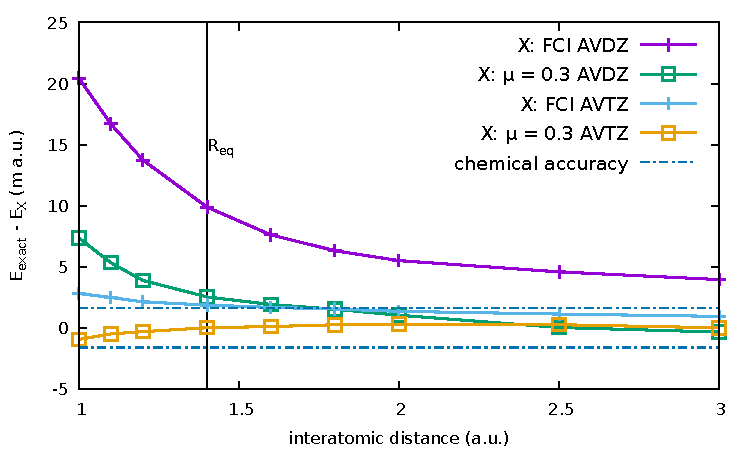
\includegraphics[width=0.45\linewidth]{plots/H2/H2_de_fci_mu_0_3.pdf}
%        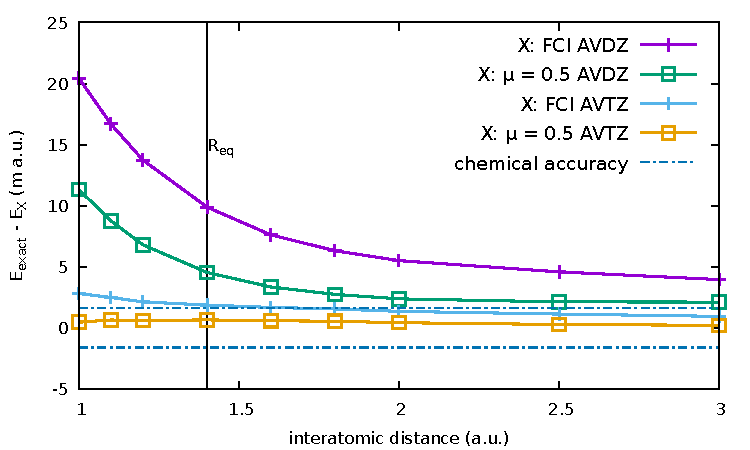
\includegraphics[width=0.45\linewidth]{plots/H2/H2_de_fci_mu_0_5.pdf}\\
%        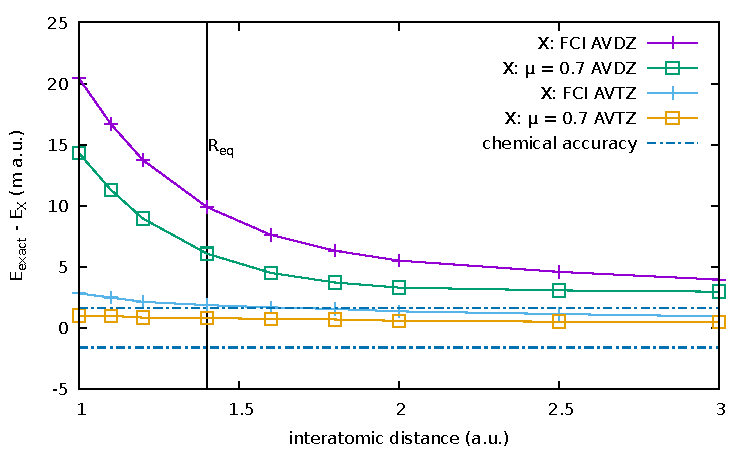
\includegraphics[width=0.45\linewidth]{plots/H2/H2_de_fci_mu_0_7.pdf}
%        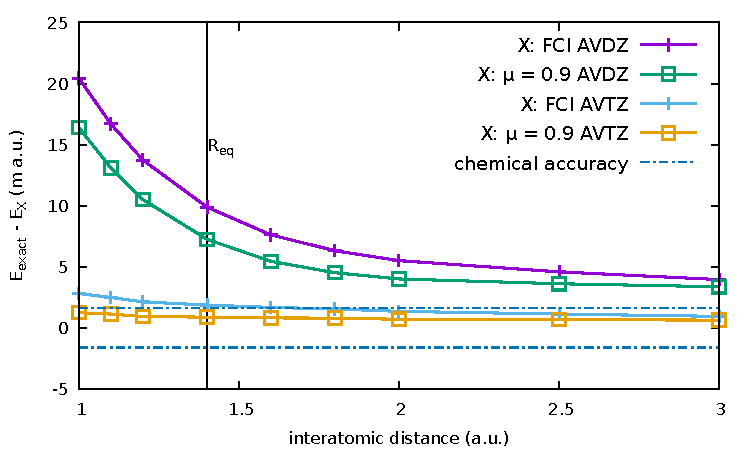
\includegraphics[width=0.45\linewidth]{plots/H2/H2_de_fci_mu_0_9.pdf}\\
%        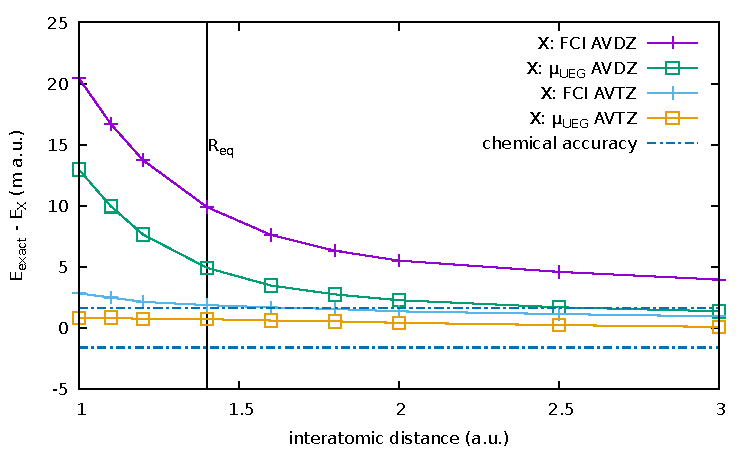
\includegraphics[width=0.45\linewidth]{plots/H2/H2_de_fci_lda.pdf}
%        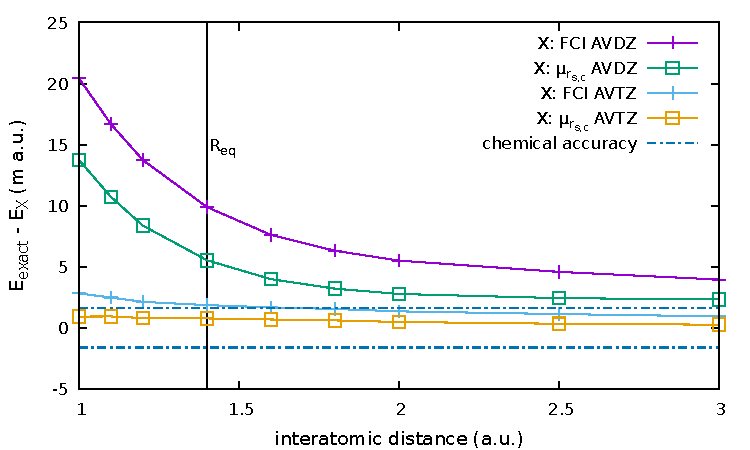
\includegraphics[width=0.45\linewidth]{plots/H2/H2_de_fci_rsc.pdf}\\
%        \caption{
%        H$_2$ molecule: Error with respect to the estimated exact ground state energy for the aug-cc-pVDZ and aug-cc-pVTZ basis sets (AVDZ, AVTZ, respectively) as a function of the inter nuclear distance for different values of $\mu$, and comparison with FCI.  
%}
%\end{figure*}

\section{Computation of integrals}
\subsection{Computation of integrals of $\hat{L}(\bri{1},\bri{2},\bri{3})$}
We need to compute the following integral 
\begin{equation}
 \label{eq:l_ijmkln}
 \begin{aligned}
 & \matelem{\phi_i \phi_k \phi_m}{\hat{L}(\bri{1},\bri{2},\bri{3})}{\phi_k \phi_l \phi_n} = \\
 & \matelem{\phi_i \phi_k \phi_m}{\hat{L}_1(\bri{1},\bri{2},\bri{3})}{\phi_k \phi_l \phi_n} \\
 & \matelem{\phi_i \phi_k \phi_m}{\hat{L}_2(\bri{1},\bri{2},\bri{3})}{\phi_k \phi_l \phi_n} \\
 & \matelem{\phi_i \phi_k \phi_m}{\hat{L}_3(\bri{1},\bri{2},\bri{3})}{\phi_k \phi_l \phi_n} 
 \end{aligned}
\end{equation}
where 
\begin{equation}
 \hat{L}_1(\bri{1},\bri{2},\bri{3}) = w_\mu(\bri{12}) w_\mu(\bri{13}) \bri{12} \cdot \bri{13}
\end{equation}
with 
\begin{equation}
 w_\mu(\bri{13}) = \frac{1 - \text{erf}(\mu r_{12})}{2 r_{12}}.
\end{equation}
Let us compute the first term of Eq. \eqref{eq:l_ijmkln}:
\begin{equation}
 \begin{aligned}
 & \matelem{\phi_i \phi_k \phi_m}{\hat{L}_1(\bri{1},\bri{2},\bri{3})}{\phi_k \phi_l \phi_n} = \\
 & \int \dr{1} \dr{2} \dr{3} \phi_i(\bri{1}) \phi_u(\bri{2}) \phi_m(\bri{3}) w_{\mu}(r_{12}) w_{\mu}(r_{13}) \\ 
 &\bri{12} \cdot \bri{13}  \phi_k(\bri{1}) \phi_l(\bri{2}) \phi_n(\bri{3}).
 \end{aligned}
\end{equation}
Such matrix element can be further decomposed into
\begin{equation}
 \begin{aligned}
 & \matelem{\phi_i \phi_k \phi_m}{\hat{L}_1(\bri{1},\bri{2},\bri{3})}{\phi_k \phi_l \phi_n}  \\
 =& \matelem{\phi_i \phi_k \phi_m}{\hat{L}_1^x(\bri{1},\bri{2},\bri{3})}{\phi_k \phi_l \phi_n} \\  
+ & \matelem{\phi_i \phi_k \phi_m}{\hat{L}_1^y(\bri{1},\bri{2},\bri{3})}{\phi_k \phi_l \phi_n} \\  
+ & \matelem{\phi_i \phi_k \phi_m}{\hat{L}_1^z(\bri{1},\bri{2},\bri{3})}{\phi_k \phi_l \phi_n},  
 \end{aligned}
\end{equation}
where 
\begin{equation}
 \begin{aligned}
 \label{eq:l_1x}
& \matelem{\phi_i \phi_k \phi_m}{\hat{L}_1^x(\bri{1},\bri{2},\bri{3})}{\phi_k \phi_l \phi_n} \\  
 = & \int \dr{1} \dr{2} \dr{3} \phi_i(\bri{1}) \phi_u(\bri{2}) \phi_m(\bri{3}) w_{\mu}(r_{12}) w_{\mu}(r_{13}) \\ 
 &(x_1 - x_2) (x_1 - x_3) \phi_k(\bri{1}) \phi_l(\bri{2}) \phi_n(\bri{3}).
 \end{aligned}
\end{equation}
If we define the following function 
\begin{equation}
 W_{mn}^x({\bf r})  = \int \text{d}{\bf r'} \phi_m({\bf r}') \phi_n({\bf r}') w_{\mu}({\bf r} - {\bf r'}) (x - x'),  
\end{equation}
it can be calculated easily by
\begin{equation}
 W_{mn}^x({\bf r})  = x \, w_{mn}({\bf r}) - w_{mn}^x({\bf r})
\end{equation}
with 
\begin{equation}
 w_{mn}({\bf r}) = \int \text{d}{\bf r'} \phi_m({\bf r}') \phi_n({\bf r}') w_{\mu}({\bf r} - {\bf r'}), 
\end{equation}
and 
\begin{equation}
  w_{mn}^x({\bf r}) = \int \text{d}{\bf r'} \phi_m({\bf r}') \phi_n({\bf r}') w_{\mu}({\bf r} - {\bf r'})  x'.
\end{equation}
Then, one can rewrite the matrix element of Eq. \eqref{eq:l_1x} as
\begin{equation}
 \begin{aligned}
 \label{eq:l_1x_2}
& \matelem{\phi_i \phi_k \phi_m}{\hat{L}_1^x(\bri{1},\bri{2},\bri{3})}{\phi_k \phi_l \phi_n} \\  
 = & \int \text{d}{\bf r} \phi_i({\bf r})  \phi_k({\bf r}) W_{mn}^x({\bf r}) W_{jl}^x({\bf r}),
 \end{aligned}
\end{equation}
which can be easily evaluated numerically. 
Therefore, the matrix element of the $\hat{L}_1(\bri{1},\bri{2},\bri{3})$ is simply 
\begin{equation}
 \begin{aligned}
 & \matelem{\phi_i \phi_k \phi_m}{\hat{L}_1(\bri{1},\bri{2},\bri{3})}{\phi_k \phi_l \phi_n} \\
 = & \int \text{d}{\bf r} \phi_i({\bf r})  \phi_k({\bf r}) \bigg( W_{mn}^x({\bf r}) W_{jl}^x({\bf r}) + W_{mn}^y({\bf r}) W_{jl}^y({\bf r}) + W_{mn}^z({\bf r}) W_{jl}^z({\bf r})\bigg),
 \end{aligned}
\end{equation}
which can be numerically evaluated easily. 
The total matrix element of the full operator is then 
\begin{equation}
 \label{eq:l_ijmkln_final}
 \begin{aligned}
 & \matelem{\phi_i \phi_k \phi_m}{\hat{L}(\bri{1},\bri{2},\bri{3})}{\phi_k \phi_l \phi_n} \\
 = & \int \text{d}{\bf r} \phi_i({\bf r})  \phi_k({\bf r}) \bigg( W_{mn}^x({\bf r}) W_{jl}^x({\bf r}) + W_{mn}^y({\bf r}) W_{jl}^y({\bf r}) + W_{mn}^z({\bf r}) W_{jl}^z({\bf r})\bigg) \\
 + & \int \text{d}{\bf r}\phi_u({\bf r})  \phi_l({\bf r}) \bigg( W_{mn}^x({\bf r}) W_{ik}^x({\bf r}) + W_{mn}^y({\bf r}) W_{ik}^y({\bf r}) + W_{mn}^z({\bf r}) W_{ik}^z({\bf r})\bigg) \\
 + & \int \text{d}{\bf r} \phi_m({\bf r})  \phi_n({\bf r}) \bigg( W_{jl}^x({\bf r}) W_{ik}^x({\bf r}) + W_{jl}^y({\bf r}) W_{ik}^y({\bf r}) + W_{jl}^z({\bf r}) W_{ik}^z({\bf r})\bigg), 
 \end{aligned}
\end{equation}
which can be computed on the fly through a simple numerical integration. 

According to Eq. \eqref{eq:comtot}, Eq. \eqref{eq:nabla_i_nabla1}, Eq. \eqref{eq:nabla_u2} and Eq. \eqref{eq:lapl_u_final}, the additional terms arising from the commutators in $\tilde{H}[u]$ are (for a two-electron system) 
\begin{equation}
 \begin{aligned}
 \label{eq:comtot2}
 & \big[ H,\hat{\tau} \big] + \frac{1}{2} \bigg[ \big[H,\hat{\tau}\big],\hat{\tau}\bigg] =  \\
 & -\frac{1}{2} 2 \times \bigg( \frac{1 - \text{erf}(\mu r_{12})}{r_{12}} - \frac{\mu}{\sqrt{\pi}} e^{-\big(\mu r_{12} \big)^2} + \frac{\bigg(1 - \text{erf}(\mu r_{12}) \bigg)^2}{4}  \bigg) \\
   &- \bigg( 1 - \text{erf}(\mu r_{12})\bigg) \deriv{}{r_{12}}{},
 \end{aligned}
\end{equation}
or equivalently
\begin{equation}
 \begin{aligned}
 \label{eq:comtot2}
 & \big[ H,\hat{\tau} \big] + \frac{1}{2} \bigg[ \big[H,\hat{\tau}\big],\hat{\tau}\bigg] =  \\
 & -\frac{1 - \text{erf}(\mu r_{12})}{r_{12}} + \frac{\mu}{\sqrt{\pi}} e^{-\big(\mu r_{12} \big)^2} - \frac{\bigg(1 - \text{erf}(\mu r_{12}) \bigg)^2}{4} \\
   & + \bigg( \text{erf}(\mu r_{12}) - 1\bigg) \deriv{}{r_{12}}{}.
 \end{aligned}
\end{equation}
Therefore, the full similarity transformed Hamiltonian can be written as
\begin{equation}
  \begin{aligned}
   \tilde{H}[u] = & \sum_{i = 1,2} \bigg( -\frac{1}{2} \big(\nabla_i\big)^2 + v(\br{}_i)  \bigg) + \frac{1}{r_{12}} \\
&   -\frac{1 - \text{erf}(\mu r_{12})}{r_{12}} + \frac{\mu}{\sqrt{\pi}} e^{-\big(\mu r_{12} \big)^2} - \frac{\bigg(1 -     \text{erf}(\mu r_{12}) \bigg)^2}{4} \\
& + \bigg( \text{erf}(\mu r_{12}) - 1\bigg) \deriv{}{r_{12}}{}
  \end{aligned}
\end{equation}
or equivalently 
\begin{equation}
  \begin{aligned}
   \tilde{H}[u] = & h_c + \frac{\text{erf}(\mu r_{12})}{r_{12}} + \frac{\mu}{\sqrt{\pi}} e^{-\big(\mu r_{12} \big)^2} - \frac{\bigg(1 -     \text{erf}(\mu r_{12}) \bigg)^2}{4} \\
& + \bigg( \text{erf}(\mu r_{12}) - 1\bigg) \deriv{}{r_{12}}{},
  \end{aligned}
\end{equation}
which corresponds precisely to Eq. \eqref{eq:h_tilde_r12}. 

\section{$r_{12} \rightarrow 0$ limits for different forms of Hamiltonians}
\label{sec:cusp}
Having established the analytical form of the transcorrelated Hamiltonian $\tilde{H}[u]$ for a general Jastrow factor $u(r_{12})$ in the case of the helium atom, one can then study the behaviour of $\tilde{H}[u]$ when $r_{12}\rightarrow 0$ and compare it to two other types of Hamiltonian: the usual physical Hamiltonian and that entering the RS-DFT framework. 
The analysis of the $r_{12}\rightarrow 0$ behaviour leads to the different condition that the eigenvectors of such operators must fulfill. For the sake of simplicity of the notations we focus on the ground state of these operators but the arguments are general for any bounded eigenvectors. 

In the case of the usual Hamiltonian, the exact ground state wave function $\psiex$ must satisfy the Schroedinger equation in real space 
\begin{equation}
 H \psiex(\br{}_1,\br{}_2) = E_0 \psiex(\br{}_1,\br{}_2)\quad \forall (\br{}_1,\br{}_2).
\end{equation}
When looking at $r_{12}\approx 0$, all terms multiplying $\frac{1}{r_{12}}$ in $H \psiex(\br{}_1,\br{}_2)$ must remain finite, which, according to Eq.\eqref{def:h_c}, translates into
\begin{equation}
 \label{eq:cusp_0}
 \lim_{r_{12}\rightarrow 0}\bigg( \frac{2}{r_{12}} \deriv{}{r_{12}}{} -\frac{1}{r_{12}}\bigg) \psiex(\bd{r_1},\bd{r_2})  = c,\quad c<\infty 
\end{equation}
or equivalently by multiplying Eq. \eqref{eq:cusp_0} by $r_{12}$
\begin{equation}
 \lim_{r_{12}\rightarrow 0}\bigg( 2 \deriv{\psiex(\bd{r_1},\bd{r_2})}{r_{12}}{} -\psiex(\bd{r_1},\bd{r_2}) \bigg) = 0, 
\end{equation}
which translates into the famous cusp condition for antiparallel spins of Kato\cite{Kat-CPAM-57}, 
\begin{equation}
 \deriv{\psiex(\bd{r_1},\bd{r_2})}{r_{12}}{}\Bigr|_{r_{12}=0} = \frac{1}{2} \psiex(r_{12}=0). 
\end{equation} 
For an excellent pedagogical and general derivation of the cusp conditions, see Ref.\onlinecite{Tew-JCP-08}. 

Regarding now the similarity transformed Hamiltonians, the exact ground state eigenvector must also satisfy an eigenvalue equation in real-space,
\begin{equation}
 \label{eq:hpi0_ex}
 \tilde{H}[u] \phiex(\br{}_1,\br{}_2) = E_0 \phiex(\br{}_1,\br{}_2) \quad \forall (\br{}_1,\br{}_2).
\end{equation}
Similarly to Eq. \eqref{eq:cusp_0}, when looking at $r_{12}\approx 0$, the terms multiplying $\frac{1}{r_{12}}$ in $\tilde{H}[u]\phiex(\br{}_1,\br{}_2)$ must remain finite, 
which involves also the term $\tilde{W}[u]$ in $\tilde{H}[u]$ (see Eq.\eqref{eq:def_wt}). Therefore, imposing the finiteness of the limit $r_{12}\rightarrow 0$ of Eq.\eqref{eq:hpi0_ex} translates into
\begin{equation}
 \label{eq:cusp_phi_0}
 \lim_{r_{12}\rightarrow 0}\bigg( \frac{2}{r_{12}} \deriv{}{r_{12}}{} -\frac{1}{r_{12}}\bigg[ 1 - 2 \deriv{u(r_{12})}{r_{12}}{}\bigg]\bigg) \phiex(\bd{r_1},\bd{r_2})  = c,\quad c<\infty.
\end{equation}
Then, the term $\frac{1}{r_{12}}\bigg[ 1 - 2\deriv{u(r_{12})}{r_{12}}{}\bigg]$ in Eq.\eqref{eq:cusp_phi_0} looks like an effective electron electron interaction induced by the presence of the Jastrow factor in $\tilde{H}[u]$. 
Therefore, as long as one imposes that 
\begin{equation}
 \label{eq:cusp_phi_1}
  \deriv{u(r_{12})}{r_{12}}{}\bigg|_{r_{12}=0} = \frac{1}{2},
\end{equation}
which is nothing but the cusp condition for the Jastrow factor $u(r_{12})$, the scalar term proportional to $\frac{1}{r_{12}}$ in Eq.\eqref{eq:cusp_phi_0} vanishes at $r_{12}=0$, and then one obtains a non-divergent effective electron-electron interaction. 
Within the condition of Eq.\eqref{eq:cusp_phi_1}, the general condition of Eq.\eqref{eq:cusp_phi_0} becomes 
\begin{equation}
 \label{eq:cusp_phi_2}
 \deriv{\phiex(\bd{r_1},\bd{r_2})}{r_{12}}{}\Bigr|_{r_{12}=0} = 0, 
\end{equation}
which implies that as long as the Jastrow factor contains the cusp conditions, the eigenfunction of $\tilde{H}[u]$ is cuspless. 
For instance, a simple Jastrow factor of the form $u(r_{12}) = \frac{1}{2} r_{12}$ releases $\phiex(\br{}_1,\br{}_2)$ from 
the constraint of fulfilling the cusp condition. 

Another form of effective Hamiltonians leading to cuspless eigenfunctions are those obtained from RS-DFT 
where the Coulomb interaction $1/r_{12}$ is split into a non-divergent long-range interaction $\text{erf}(\mu r_{12})/r_{12}$ and a complementary short-range interaction $\text{erfc}(\mu r_{12})/r_{12}$, where $\text{erf}(x)$ and $\text{erfc}(x)$ are the error and complementary error functions, respectively. 
The parameter which controls such a splitting is the so-called range separation parameter $\mu$:  RS-DFT reduces the usual WFT when $\mu \rightarrow \infty$, and $\mu \rightarrow 0$ it gives back the usual Kohn-Sham theory.  
In practice, RS-DFT introduces a self-consistent Schroedinger-like equation which must be fulfilled by an effective wave function  $\Psi^\mu$.
Applied to a two electron system and looking in regions where $r_{12}\approx 0$, the leading terms of the self-consistent Schroedinger-like equation of RS-DFT reads 
\begin{equation}
 \label{eq:cusp_psi_mu_0}
 \lim_{r_{12}\rightarrow 0}\bigg( \frac{2}{r_{12}} \deriv{}{r_{12}}{} -\frac{\text{erf}(\mu r_{12})}{r_{12}}\bigg) \Psi^\mu(\bd{r_1},\bd{r_2})  = c,\quad c<\infty,  
\end{equation}
and as the effective interaction $\frac{\text{erf}(\mu r_{12})}{r_{12}}$ is non divergent at $r_{12}=0$ for finite values of $\mu$
\begin{equation}
 \lim_{r_{12} \rightarrow 0} \frac{\text{erf}(\mu r_{12})}{r_{12}} = \frac{2 \mu}{\sqrt{\pi}} , 
\end{equation}
one obtains that 
\begin{equation}
 \label{eq:cusp_psi_mu_1}
 \deriv{\Psi^\mu(\bd{r_1},\bd{r_2})}{r_{12}}{}\Bigr|_{r_{12}=0} = 0, 
\end{equation}
which means that the wave functions $\Psi^\mu$, just as $\phiex$ are cuspless, because they deal with an effective non-divergent interaction. 

Therefore, one can see that there is a similarity between the eigenvectors of RS-DFT and of the transcorrelated Hamiltonian: they are both cuspless as they originate from non divergent Hamiltonians. 

\section{Integrals involved in TenNo work}
The Jastrow factor of Ten-No is of the form
\begin{equation}
 u(r_{12})=\sum_{m=1}^{N_g} c_m e^{-\alpha_m \big(r_{12}\big)^2},
\end{equation}
where the $c_m$ and $\alpha_m$ are given in \cite{TenNo-CPL-00-a}. 
To compute the transcorrelated Hamiltonian one needs to compute therefore 
\begin{equation}
 \begin{aligned}
 \label{def_k}
  \hat{K}(\bri{1},\bri{2}) ) = \frac{1}{2} \bigg( &\nabla_1^2 u(\bri{1},\bri{2}) + \nabla_2^2u(\bri{1},\bri{2}) \\
                                               + &\big(\nabla_1 u(\bri{1},\bri{2}) \big) ^2 + \big(\nabla_1 u(\bri{1},\bri{2}) \big) ^2 \bigg) \\
                                               + &\nabla_1 u(\bri{1},\bri{2}) \cdot \nabla_2 + \nabla_2 u(\bri{1},\bri{2}) \cdot \nabla_1.
 \end{aligned}
\end{equation}
\subsection{Computation of the gradient}
One can write that 
\begin{equation}
 u(r_{12})=\sum_{m=1}^{N_g} c_m v(r_{12},\alpha_m)
\end{equation}
with 
\begin{equation}
 v(r_{12},\alpha) = e^{-\alpha \big(r_{12}\big)^2}.
\end{equation}
The gradient with respect to $\br{1}$ is 
\begin{equation}
 \deriv{}{x_1}{} v(r_{12},\alpha) = -2 \alpha (x_1 - x_2) e^{-\alpha \big(r_{12}\big)^2},
\end{equation}
and one has of course 
\begin{equation}
 \deriv{}{x_2}{} v(r_{12},\alpha) = - \deriv{}{x_1}{} v(r_{12},\alpha). 
\end{equation}
\subsection{Computation of the non Hermitian term}
One needs to compute 
\begin{equation}
 \nabla_1 v(r_{12},\alpha) \cdot \nabla_1 + \nabla_2 v(r_{12},\alpha) \cdot \nabla_2,
\end{equation}
but as 
\begin{equation}
 \deriv{}{x_2}{} v(r_{12},\alpha) = - \deriv{}{x_1}{} v(r_{12},\alpha), 
\end{equation}
one has 
\begin{equation}
  \nabla_1 v(r_{12},\alpha) \cdot \nabla_1 + \nabla_2 v(r_{12},\alpha) \cdot \nabla_2 = \nabla_1 u(r_{12},\alpha) \cdot  \big( \nabla_1 - \nabla_2 \big). 
\end{equation}
Let us introduce the following functions  
\begin{equation}
 w_{ij}(\alpha,\bri{1}) = \int \text{d}\br{} e^{-\alpha \big(\br{} - \bri{1} \big)^2} \phi_i(\br{}) \phi_j(\br{}),
\end{equation}
\begin{equation}
 w_{ij}^x(\alpha,\bri{1}) = \int \text{d}\br{}  e^{-\alpha \big(\br{} - \bri{1} \big)^2} x\phi_i(\br{}) \phi_j(\br{}).
\end{equation}
Therefore, the integral of the form 
\begin{equation}
 \begin{aligned}
 \matelem{kl}{\nabla_1 u(\bri{1},\bri{2}) \cdot  \big( \nabla_1 - \nabla_2 \big)}{ij} = \int \text{d}\bri{1}  \text{d}\bri{2}  \phi_k(\bri{1}) \phi_l(\bri{2}) \\
\nabla_1 u(\bri{1},\bri{2}) \cdot  \big( \nabla_1 - \nabla_2 \big)  \phi_i(\bri{1}) \phi_j(\bri{2}) ,
 \end{aligned}
\end{equation}
can be put into 
\begin{equation}
 \begin{aligned}
 \matelem{kl}{\nabla_1 u(\bri{1},\bri{2}) \cdot  \big( \nabla_1 - \nabla_2 \big)}{ij} = \matelem{kl}{\hat{t}_x(\alpha) + \hat{t}_y(\alpha) + \hat{t}_z(\alpha)}{ij},
 \end{aligned}
\end{equation}
with 
\begin{equation}
 \begin{aligned}
 \matelem{kl}{\hat{t}_x(\alpha)}{ij} =&  -2 \alpha \int \text{d}\bri{1} \phi_k(\bri{1}) x_1\big( \deriv{}{x_1}{} \phi_i(\bri{1})\big) w_{jl}(\alpha,\bri{1})  \\
                                      &  -2 \alpha \int \text{d}\bri{1} \phi_l(\bri{1}) x_1\big( \deriv{}{x_1}{} \phi_j(\bri{j})\big) w_{ik}(\alpha,\bri{1})  \\
                                      &  +2 \alpha \int \text{d}\bri{1} \phi_k(\bri{1}) \big( \deriv{}{x_1}{} \phi_i(\bri{j})\big) w_{jl}^x(\alpha,\bri{1})  \\
                                      &  +2 \alpha \int \text{d}\bri{1} \phi_l(\bri{1}) \big( \deriv{}{x_1}{} \phi_j(\bri{j})\big) w_{ik}^x(\alpha,\bri{1})  \\
 \end{aligned}
\end{equation}
\subsection{Computation of the square term}
One needs to compute 
\begin{equation}
 \begin{aligned}
 \bigg( \nabla_1 u(r_{12}) \bigg)^2 = \sum_{m,n=1}^{N_g} c_m c_n \nabla_1 v(r_{12},\alpha_m) \cdot \nabla_1 v(r_{12},\alpha_n).
 \end{aligned}
\end{equation}
The term $\nabla_1 v(r_{12},\alpha_m) \cdot \nabla_1 v(r_{12},\alpha_n)$ is 
\begin{equation}
 \nabla_1 v(r_{12},\alpha_m) \cdot \nabla_1 v(r_{12},\alpha_n) = 4 \alpha_m \alpha_n v(r_{12}, \alpha_m + \alpha_n) (\bri{1}- \bri{2})^2.
\end{equation}
Therefore, the integral of type 
\begin{equation}
 \matelem{kl}{\bigg( \nabla_1 u(r_{12}) \bigg)^2}{ij} = \int \text{d}\bri{1}  \text{d}\bri{2} \phi_i(\bri{1}) \phi_j(\bri{2}) \phi_k(\bri{1}) \phi_l(\bri{2}) \big(\nabla_1 u(r_{12}) \big)^2
\end{equation}
can be written as  
\begin{equation}
 \matelem{kl}{\bigg( \nabla_1 u(r_{12}) \bigg)^2}{ij} = \sum_{m,n=1}^{N_g} c_m c_n  4 \alpha_m \alpha_n \matelem{kl}{v(r_{12}, \alpha_m + \alpha_n) (\bri{1}- \bri{2})^2}{ij} 
\end{equation}
where 
\begin{equation}
 \begin{aligned}
 &\matelem{kl}{v(r_{12}, \alpha_m + \alpha_n) (\bri{1}- \bri{2})^2}{ij} \\& = \matelem{kl}{I_x(\alpha_m + \alpha_n) + I_y(\alpha_m + \alpha_n) + I_z(\alpha_m + \alpha_n)}{ij}
 \end{aligned}
\end{equation}
where 
\begin{equation}
 \begin{aligned}
 \matelem{kl}{I_x(\alpha)}{ij}=& \int \text{d}\bri{1} \phi_i(\bri{1}) \phi_k(\bri{1}) (x_1)^2 w_{jl}(\alpha,\bri{1}) \\
                              +& \int \text{d}\bri{1} \phi_j(\bri{1}) \phi_l(\bri{1}) (x_1)^2 w_{ik}(\alpha,\bri{1}) \\
                              -& \int \text{d}\bri{1} \phi_i(\bri{1}) \phi_k(\bri{1}) x_1 w_{jl}^x(\alpha,\bri{1}) \\
                              -& \int \text{d}\bri{1} \phi_j(\bri{1}) \phi_l(\bri{1}) x_1 w_{ik}^x(\alpha,\bri{1}) \\
 \end{aligned}
\end{equation}
\subsection{Computation of the Laplacian}
One needs to compute 
\begin{equation}
 \begin{aligned}
  \Delta_1 u(r_{12}) = \sum_{m} c_m \Delta_1  v(r_{12},\alpha_m).
 \end{aligned}
\end{equation}
The Laplacian of $v(r_{12},\alpha)$ is 
\begin{equation}
 \begin{aligned}
 \deriv{}{x_1}{2} v(r_{12},\alpha) &= \deriv{}{x_2}{2} v(r_{12},\alpha) \\
                           &= v(r_{12},\alpha) 2 \alpha \bigg( 2 \alpha \big( (x_1)^2 + (x_2)^2 \big) -4 \alpha x_1 x_2  -1\bigg)
 \end{aligned}
\end{equation}
and so 
\begin{equation}
 \begin{aligned}
 \Delta_1 v(r_{12},\alpha) &= v(r_{12},\alpha) 2 \alpha \bigg( 2 \alpha \big( (r_1)^2 + (r_2)^2 \big) -4 \alpha \bri{1}\cdot \bri{2}  -3\bigg).
 \end{aligned}
\end{equation}
One can express the following integral 
\begin{equation}
 \matelem{kl}{\Delta_1 v(r_{12},\alpha)}{ij} = \int \text{d}\bri{1}  \text{d}\bri{2} \Delta_1 v(r_{12},\alpha) 
\phi_i(\bri{1}) \phi_j(\bri{2}) \phi_k(\bri{1}) \phi_l(\bri{2}),
\end{equation}
as 
\begin{equation}
 \begin{aligned}
  \matelem{kl}{\Delta_1 v(r_{12},\alpha)}{ij} =&  4 \alpha^2 \int \text{d}\bri{1} (r_1)^2 \phi_i(\bri{1}) \phi_k(\bri{1}) w_{jl}(\alpha,\bri{1})  \\
                                               +& 4 \alpha^2 \int \text{d}\bri{1} (r_1)^2 \phi_j(\bri{1}) \phi_l(\bri{1}) w_{ik}(\alpha,\bri{1})  \\
                                               -& 6 \alpha \int \text{d}\bri{1} \phi_j(\bri{1}) \phi_l(\bri{1}) w_{ik}(\alpha,\bri{1})  \\
                                               -& 8 \alpha^2 \int \text{d}\bri{1} x_1 \phi_j(\bri{1}) \phi_l(\bri{1}) w_{ik}^x(\alpha,\bri{1})  \\
                                               -& 8 \alpha^2 \int \text{d}\bri{1} y_1 \phi_j(\bri{1}) \phi_l(\bri{1}) w_{ik}^y(\alpha,\bri{1})  \\
                                               -& 8 \alpha^2 \int \text{d}\bri{1} z_1 \phi_j(\bri{1}) \phi_l(\bri{1}) w_{ik}^z(\alpha,\bri{1})  \\
 \end{aligned}
\end{equation}


\section{Numerical computation of integrals}
\subsection{Fit of functions}
\subsubsection{Fit of $1-\text{erf}(x)$}
At some point we would like to fit the following function
\begin{equation}
 g(x) = 1-\text{erf}(x)
\end{equation}
which can be done, for instance by 
\begin{equation}
 h(x,\alpha,\beta,c) = e^{-\alpha x - \beta x^2}
\end{equation}
with $\alpha=1.09529$ and $\beta = 0.756023$. 
So by posing $y=\mu x$, $x=y/\mu$ then
\begin{equation}
 \label{fit_erf}
 \begin{aligned}
  g(x,\mu)  =& 1 - \text{erf}(\mu x) \approx e^{-\alpha \mu x - \beta (\mu x)^2}\\ 
        =& e^{-\alpha \mu x } e^{-\beta \mu^2 x^2} \\
        =& h(x,\alpha \mu, \beta \mu^2).
 \end{aligned}
\end{equation}
Therefore, one can fit $g(x)^2$ as 
\begin{equation}
 \begin{aligned}
 g(x,\mu)^2 = \bigg( 1 - \text{erf}(\mu x) \bigg)^2\\
           &= \bigg( e^{-\alpha \mu x } e^{-\beta \mu^2 x^2}\bigg)^2 \\
           &= e^{-2\alpha  \mu x } e^{-2 \beta \mu^2 x^2} \\
           &= h(x,2 \alpha \mu, 2 \beta \mu^2).
 \end{aligned}
\end{equation}

\subsubsection{Fit of $e^{-x}$}
The fit of $1 - \text{erf}(\mu x)$ in Eq. \eqref{fit_erf} involves a Slater function, which is always rather complex to integrate. 
Nevertheless, we can fit a Slater function with Gaussian functions (that is what quantum chemistry is about):
\begin{equation}
 e^{-X} = \sum_{m=1}^{N_s} c_m e^{-\zeta_m X^2}, 
\end{equation}
and, by posing $X=\gamma x$ one can fit any Slater function as
\begin{equation}
 e^{-\gamma x} = \sum_{m=1}^{N_s} c_m e^{-\zeta_m \gamma^2 x^2}. 
\end{equation}
To find the $\{c_m,\zeta_m\}$ parameters, I performed a Hartree Fock calculation on the Hydrogen atom using the $s$ functions of the ANO-RCC basis set which contains 8 gaussians.  

\subsection{Computation of integrals with $\text{exp}(-\alpha r_{12}^2)$}
As essentially all functions of $r_{12}$ involve directly or indirectly (\textit{i.e.} through a fit) gaussian functions, we will have to evaluate such integrals
\begin{equation}
 \begin{aligned}
  \int \text{d}\br{}_1  \text{d}\br{}_2& \big( x_1 - A_x \big)^{a_x}  \big( x_2 - B_x \big)^{b_x} 
                                         \big( y_1 - A_y \big)^{a_y}  \big( y_2 - B_y \big)^{b_y} 
                                         \big( z_1 - A_z \big)^{a_z}  \big( z_2 - B_z \big)^{b_z} \\
                                       & \text{exp}(-\alpha \big(\br{}_1 - {\bf A} \big)^2)
                                         \text{exp}(-\beta  \big(\br{}_2 - {\bf B} \big)^2)
                                         \text{exp}(-\delta \big(\br{}_1 - \br{}_2 \big)^2)
 \end{aligned}
\end{equation}
which can be transformed into product of types 
\begin{equation}
 \begin{aligned}
  \int \text{d}x_1 \text{d}x_2 & \big( x_1 - A_x \big)^{a_x} \big( x_2 - B_x \big)^{b_x} \\ 
  & \text{exp}(-\alpha \big(x_1 - A_x \big)^2) \text{exp}(-\alpha \big(x_2 - B_x \big)^2) \text{exp}(-\delta \big(x_1 - x_2 \big)^2)
 \end{aligned}
\end{equation}

\section{New form of jastrow factor}
We want the jastrow factor $u(r_{12})$ to fulfil such equation
\begin{equation}
 - \bigg[ \frac{2}{r_{12}} \deriv{u}{r_{12}}{}  + \deriv{u}{r_{12}}{2} \bigg] + \frac{1}{r_{12}} = \frac{\text{erf}\big( \mu r_{12} \big)}{r_{12}}.
\end{equation}
The solution for such an equation is 
\begin{equation}
 u(r_{12}) = \frac{1}{2}r_{12}\bigg( 1 - \text{erf}(\mu r_{12}) \bigg) - \frac{1}{2\sqrt{\pi} \mu} e^{-\big( \mu r_{12}\big)^2} + \frac{1}{4 r_{12}} \bigg(c_1 - \frac{\text{erf}\big(\mu r_{12} \big)}{\mu^2} \bigg).
\end{equation}
The constant $c_1$ can be found to impose that 
\begin{equation}
 \lim_{r_{12} \rightarrow 0 } u(r_{12}) < \infty,
\end{equation}
which means $c_1 = 0$. Therefore the new jastrow factor is 
\begin{equation}
 u(r_{12}) = \frac{1}{2}r_{12}\bigg( 1 - \text{erf}(\mu r_{12}) \bigg) - \frac{1}{2\sqrt{\pi} \mu} e^{-\big( \mu r_{12}\big)^2}  - \frac{\text{erf}\big(\mu r_{12} \big)}{4 \mu^2 r_{12}}.
\end{equation}

\section{One body term jastrow}
\subsection{The case of the Hydrogen atom}
We want to find a Jastrow factor which will take care of the nuclear-electron cusp condition, and we will begin by the Hydrogen atom.  

Let us write the Hamiltonian of the hydrogenoid atom in the radial coordinate for the $l=0$ sector 
\begin{equation}
 H = -\frac{1}{2} \big( \deriv{}{r}{2} + \frac{2}{r} \deriv{}{r}{}\big) - \frac{Z}{r}.
\end{equation}
To do so, we have to compute the kinetic part acting on the Jastrow factor acting on a function depending only on the radial coordinate $\phi( r)$
\begin{equation}
 \label{eq:h_atom_j}
 \begin{aligned}
 & -\frac{1}{2}e^{-u(r)}\big(\deriv{}{r}{2} + \frac{2}{r} \deriv{}{r}{} \big) e^{u(r)}\phi(r)  = \\
 & -\frac{1}{2}\big( \deriv{}{r}{2} + \frac{2}{r} \deriv{}{r}{} \big) \phi(r) \\
 &-\deriv{u(r)}{r}{}\deriv{}{r}{}\phi(r) \\
 &-\frac{1}{r}\deriv{u(r)}{r}{}\phi(r)  - \frac{1}{2}\deriv{u(r)}{r}{2}\phi(r)  -  \frac{1}{2}\bigg(\deriv{u(r)}{r}{} \bigg)^2 \phi(r).
 \end{aligned}
\end{equation}
Therefore the full similarity transformed Hamiltonian $\tilde{H}[u]$ is 
\begin{equation}
 \begin{aligned}
 \label{eq:one_e_0}
 & e^{-u(r)}H\,e^{u(r)} = \\
 & -\frac{1}{2}\big( \deriv{}{r}{2} + \frac{2}{r} \deriv{}{r}{} \big) -\deriv{u(r)}{r}{}\deriv{}{r}{}\\
 &-\frac{1}{r}\bigg(\deriv{u(r)}{r}{} + Z \bigg) \\ 
 & - \frac{1}{2}\deriv{u(r)}{r}{2} -  \frac{1}{2}\bigg(\deriv{u(r)}{r}{} \bigg)^2.
 \end{aligned}
\end{equation}
Similarly to what have been proposed in Section \ref{sec:he_j}, we want to find the Jastrow factor $u(r,\mu,Z)$ such that 
\begin{equation}
 \label{eq:one_e_01}
 -\frac{1}{r}\bigg(\deriv{u(r,\mu,Z)}{r}{} + Z \bigg) = -Z\frac{\text{erf}(\mu r)}{r},
\end{equation}
or equivalently
\begin{equation}
 \label{eq:one_e_1}
 \deriv{}{r}{}u(r,\mu,Z) = Z\bigg( \text{erf}(\mu r) - 1\bigg).
\end{equation}
The Jastrow factor fulfilling Eq. \eqref{eq:one_e_1} is 
\begin{equation}
 \label{eq:one_e_2}
 u(r,\mu,Z) = -Z r \bigg( 1 - \text{erf}\big(\mu r\big) \bigg) + \frac{Z}{\sqrt{\pi}\mu} e^{-\big(\mu r \big)^2}. 
\end{equation}
Now, we can plug $u(r,\mu,Z)$ into Eq. \eqref{eq:one_e_0} in order to compute the explicit form of the similarity transformed Hamiltonian. 
To do so, we use Eq. \eqref{eq:one_e_1}, and also that 
\begin{equation}
 \deriv{}{r}{2}u(r) = \frac{2 \mu Z }{\sqrt{\pi}} e^{-(\mu r)^2}.
\end{equation}
One obtains then the similarity transformed Hamiltonian 
\begin{equation}
 \begin{aligned}
 \tilde{H}[u] = & e^{-u(r)} H e^{u(r)} \\
              = & -\frac{1}{2}\big( \deriv{}{r}{2} + \frac{2}{r} \deriv{}{r}{} \big) - \frac{Z}{r}  \\
                & + Z \bigg( 1 - \text{erf}(\mu r)\bigg) \deriv{}{r}{} \\
                & - Z \frac{\text{erf}(\mu r) - 1}{r} \\
                & -Z \frac{\mu}{\sqrt{\pi}} e^{-(\mu r)^2} \\
                & - \frac{1}{2}Z^2 \bigg( \text{erf}(\mu r) -1 \bigg)^2,
 \end{aligned}
\end{equation}
and one can notice that the $\frac{-Z}{r}$ interaction cancels out to give
\begin{equation}
 \label{eq:one_e_3}
 \begin{aligned}
 \tilde{H}[u] = & e^{-u(r)} H e^{u(r)} \\
              = & -\frac{1}{2}\big( \deriv{}{r}{2} + \frac{2}{r} \deriv{}{r}{} \big)  \\
                & -Z \bigg[ \frac{\mu}{\sqrt{\pi}} e^{-(\mu r)^2} + \frac{\text{erf}(\mu r)}{r} + \frac{1}{2}Z \bigg( \text{erf}(\mu r) -1 \bigg)^2 \bigg] \\
                & + Z \bigg( 1 - \text{erf}(\mu r)\bigg) \deriv{}{r}{}. 
 \end{aligned}
\end{equation}
Therefore, compared to the usual Hamiltonian, the similarity transformed Hamiltonian contains a different local interaction which is clearly non divergent, but also a new short-range differential operator. 

\subsection{General equation}
Now that we know the general form of the one-body Jastrow factor for a one electron system, we can generalize it 
to an $N$-electron system and an $M$ nucleus system by just taking the following form 
\begin{equation}
 e^{\hat{\tau}({\bf r}_1,\hdots , {\bf r}_i,{\bf r}_N)} = e^{-\sum_i^N u({\bf r}_i)} 
\end{equation}
where $u({\bf r}_i)$ has the following form 
\begin{equation}
 u({\bf r}_i) = \sum_{A} u(r_{iA},\mu,Z_A) 
\end{equation}
where $u(r,\mu,Z)$ is given by Eq. \eqref{eq:one_e_2} and $r_{iA} = \big|{\bf r}_i - {\bf R}_A \big|$. 
According to Eq. (2) of Ref. \onlinecite{CohLuoGutDobTewAla-JCP-19}, the equation of the similarity transformed Hamiltonian is similar  
to that of Eq. \eqref{ht_def_g} but with a new form of Jastrow factor. 
Therefore one needs to compute $\big[ H,\hat{\tau} \big]$ and $\frac{1}{2}\bigg[ \big[H,\hat{\tau}\big],\hat{\tau}\bigg]$. 
Let us begin by $\big[ H,\hat{\tau} \big]$, and as before, we apply it to a general function $\phi(\br{}_1,\hdots \br{}_N)$:
\begin{equation}
 \label{eq:one_com1_1}
 \begin{aligned}
 \bigg[ H, \hat{\tau} \bigg]\phi(\br{}_1,\hdots \br{}_N) & = \bigg[ -\frac{1}{2} \sum_i \nabla^2_i, \sum_{u} u(\br{}_j) \bigg]      \phi(\br{}_1,\hdots \br{}_N) \\    
                                                        & = -\frac{1}{2} \sum_i \bigg( \big(\nabla^2_i u({\bf r}_i)\big) + 2\nabla_i u({\bf r}_i) \cdot \nabla_i \phi(\br{}_1,\hdots \br{}_N) \bigg).  
 \end{aligned}
\end{equation}
Therefore, one can write that term as
\begin{equation}
 \label{eq:one_com1_2}
 \begin{aligned}
  \big[ H,\hat{\tau} \big] =& -\frac{1}{2} \bigg( \sum_i \nabla^2_i u(\br{}_i) \bigg) \\
                            & -\sum_i \bigg(\nabla_i u(\br{}_i) \bigg) \cdot \bigg( \nabla_i  \bigg).
 \end{aligned}
\end{equation}
After some math, the second-order commutator is simply 
\begin{equation}
 \bigg[ \big[H,\hat{\tau}\big],\hat{\tau}\bigg] = -\sum_i \nabla_i u({\bf r}_i) \cdot \nabla_i u({\bf r}_i) 
\end{equation}
So eventually, the similarity transformed operator becomes 
\begin{equation}
 \begin{aligned}
& H + \big[ H,\hat{\tau} \big] + \frac{1}{2} \bigg[ \big[H,\hat{\tau}\big],\hat{\tau}\bigg] = \\ & H -\frac{1}{2} \bigg( \sum_i \nabla^2_i u(\br{}_i) \bigg)    
                                                                   -\sum_i \bigg(\nabla_i u(\br{}_i) \bigg) \cdot \bigg( \nabla_i  \bigg)  
                                                                   -\frac{1}{2}\sum_i \nabla_i u({\bf r}_i) \cdot \nabla_i u({\bf r}_i) 
 \end{aligned}
\end{equation}
Therefore, the addition of the jastrow operator does not add extra two-body terms. 
\subsection{Computation of the total operator}
\subsubsection{Computation of $\nabla_i u(\br{}_i)$}
\begin{equation}
 \begin{aligned}
&\nabla_i u(\br{}_i) = \sum_A \nabla_i u(r_{iA},Z_A) \\
                    &= \sum_A \deriv{}{x_i}{} u(r_{iA},Z_A) {\bf e}_{x_i} + \deriv{}{y_i}{} u(r_{iA},Z_A) {\bf e}_{y_i} + \deriv{}{z_i}{} u(r_{iA},Z_A) {\bf e}_{z_i}, 
 \end{aligned}
\end{equation}
and 
\begin{equation}
 \deriv{}{x_i}{}u(r_{iA}) = \deriv{}{r_{iA}}{}u(r_{iA}) \deriv{r_{iA}}{x_i}{},
\end{equation}
and as $r_{iA} = \sqrt{(x_1 - x_A)^2 + (y_1 - y_A)^2 + (z_1 - z_A)^2} $ 
one has                                                              
\begin{equation}
 \deriv{r_{iA}}{x_1}{} = \frac{x_1 - x_A}{r_{iA}}
\end{equation}
and therefore according to Eq. \eqref{eq:one_e_1}, one has 
\begin{equation}
 \deriv{}{x_i}{} u(r_{iA},Z_A) = -\sum_A Z_A \big( x_i - x_A \big) \frac{1 - \text{erf}(\mu r_{iA})}{r_{iA}}.
\end{equation}
\subsubsection{Computation of $\nabla_i u({\bf r}_i) \cdot \nabla_i u({\bf r}_i)$}
The computation of $\nabla_i u({\bf r}_i) \cdot \nabla_i u({\bf r}_i)$ leads to 
\begin{equation}
 \begin{aligned}
  \nabla_i u({\bf r}_i) \cdot \nabla_i u({\bf r}_i) =  \sum_{A,B} Z_B &Z_A \big( x_i - x_A \big) \big( x_i - x_B \big)  \frac{ 1 -\text{erf}(\mu r_{iA})}{r_{iA}} \frac{ 1 - \text{erf}(\mu r_{iB})}{r_{iB}} \\
                                                                      & +  \big( y_i - y_A \big) \big( y_i - y_B \big)  \frac{ 1 -\text{erf}(\mu r_{iA})}{r_{iA}} \frac{ 1 - \text{erf}(\mu r_{iB})}{r_{iB}} \\ 
                                                                      & +  \big( z_i - z_A \big) \big( z_i - z_B \big)  \frac{ 1 -\text{erf}(\mu r_{iA})}{r_{iA}} \frac{ 1 - \text{erf}(\mu r_{iB})}{r_{iB}}.
 \end{aligned}
\end{equation}
The diagonal part of such integrals is simply
\begin{equation}
 \begin{aligned}
 &  \sum_{A} (Z_A)^2 \bigg(\big( x_i - x_A \big)^2 +  \big( y_i - y_A \big)^2 + \big( z_i - z_A \big)^2\bigg) \frac{\bigg(\text{erf}(\mu r_{iA}) - 1\bigg)^2}{\big(r_{iA}\big)^2}\\ 
  = & \sum_{A} (Z_A)^2 \bigg( \text{erf}(\mu r_{iA}) -1 \bigg)^2
 \end{aligned}
\end{equation}


\subsubsection{Computation of $\nabla^2_i u(\br{}_i) $}
We need to compute 
\begin{equation}
 \begin{aligned}
 \deriv{}{x_{i}}{2} u(\br{}_i) & = -\sum_A Z_A \deriv{}{x_i}{} \bigg[(x_i - x_A) \frac{1 - \text{erf}(\mu r)}{r_{iA}} \bigg] \\
                               & = -\sum_A Z_A \bigg[ \frac{1 - \text{erf}(\mu r_{iA})}{r_{iA}} + (x_i - x_A) \deriv{}{x_i}{}\frac{1 - \text{erf}(\mu r_{iA})}{r_{iA}}  \bigg]
 \end{aligned}
\end{equation}
But, one has that
\begin{equation}
 \begin{aligned}
 \deriv{}{x_i}{} \frac{1 - \text{erf}(\mu r_{iA})}{r_{iA}} = - \frac{(x_i - x_A)}{(r_{iA})^2} \bigg( \frac{2 \mu}{\sqrt{\pi}} e^{-(\mu r_{iA})^2} + \frac{1 - \text{erf}(\mu r_{iA})}{r_{iA}}\bigg).
 \end{aligned}
\end{equation}
Therefore, 
\begin{equation}
 \label{eq:lapl_important}
 (x_i - x_A) \deriv{}{x_i}{}\frac{1 - \text{erf}(\mu r_{iA})}{r_{iA}} = - \frac{(x_i - x_A)^2}{(r_{iA})^2} \bigg( \frac{2 \mu}{\sqrt{\pi}} e^{-(\mu r_{iA})^2} + \frac{1 - \text{erf}(\mu r_{iA})}{r_{iA}}\bigg)
\end{equation}.
Therefore, the Laplacian is 
\begin{equation}
 \begin{aligned}
 \label{eq:lapl_interm_1}
&  \deriv{}{x_{i}}{2} u(\br{}_i) + \deriv{}{y_{i}}{2} u(\br{}_i) + \deriv{}{z_{i}}{2} u(\br{}_i) =  - \sum_{A} Z_A \bigg[ 3 \frac{1 - \text{erf}(\mu r_{iA})}{r_{iA}}  \\
 & + (x_i - x_A) \deriv{}{x_i}{}\frac{1 - \text{erf}(\mu r_{iA})}{r_{iA}} \\ 
 & + (y_i - y_A) \deriv{}{y_i}{}\frac{1 - \text{erf}(\mu r_{iA})}{r_{iA}} \\ 
 & + (z_i - z_A) \deriv{}{z_i}{}\frac{1 - \text{erf}(\mu r_{iA})}{r_{iA}}  \bigg]
 \end{aligned}
\end{equation}
But according to Eq. \eqref{eq:lapl_important}, one has that 
\begin{equation}
 \begin{aligned}
 & + (x_i - x_A) \deriv{}{x_i}{}\frac{1 - \text{erf}(\mu r_{iA})}{r_{iA}} \\ 
 & + (y_i - y_A) \deriv{}{y_i}{}\frac{1 - \text{erf}(\mu r_{iA})}{r_{iA}} \\ 
 & + (z_i - z_A) \deriv{}{z_i}{}\frac{1 - \text{erf}(\mu r_{iA})}{r_{iA}}  = \\
 &- \frac{(x_i - x_A)^2 + (y_i - y_A)^2 + (z_i - z_A)^2}{(r_{iA})^2} \bigg( \frac{2 \mu}{\sqrt{\pi}} e^{-(\mu r_{iA})^2} + \frac{1 - \text{erf}(\mu r_{iA})}{r_{iA}}\bigg)
 \end{aligned}
\end{equation}
which is simply 
\begin{equation}
 \begin{aligned}
 \label{eq:lapl_interm_2}
 & + (x_i - x_A) \deriv{}{x_i}{}\frac{1 - \text{erf}(\mu r_{iA})}{r_{iA}} \\ 
 & + (y_i - y_A) \deriv{}{y_i}{}\frac{1 - \text{erf}(\mu r_{iA})}{r_{iA}} \\ 
 & + (z_i - z_A) \deriv{}{z_i}{}\frac{1 - \text{erf}(\mu r_{iA})}{r_{iA}}  = \\
 &- \bigg( \frac{2 \mu}{\sqrt{\pi}} e^{-(\mu r_{iA})^2} + \frac{1 - \text{erf}(\mu r_{iA})}{r_{iA}}\bigg).
 \end{aligned}
\end{equation}
Then, coming back to Eq. \eqref{eq:lapl_interm_1} with Eq. \eqref{eq:lapl_interm_2} one has 
\begin{equation}
 \Delta_i u(\br{}_i) = - \sum_{A}  Z_A \bigg[ 3 \frac{1 - \text{erf}(\mu r_{iA})}{r_{iA}}  - \bigg( \frac{2 \mu}{\sqrt{\pi}} e^{-(\mu r_{iA})^2} + \frac{1 - \text{erf}(\mu r_{iA})}{r_{iA}}\bigg) \bigg]
\end{equation}
which becomes 
\begin{equation}
 \Delta_i u(\br{}_i) = - \sum_{A}  2 \, Z_A  \bigg[ \frac{1 - \text{erf}(\mu r_{iA})}{r_{iA}}  - \frac{\mu}{\sqrt{\pi}} e^{-(\mu r_{iA})^2}  \bigg]
\end{equation}
\subsubsection{Computation of the total operator}
\begin{equation}
 \begin{aligned}
& H + \big[ H,\hat{\tau} \big] + \frac{1}{2} \bigg[ \big[H,\hat{\tau}\big],J\bigg] = \\ & H -\frac{1}{2} \bigg( \sum_i \nabla^2_i u(\br{}_i) \bigg)    
                                                                   -\sum_i \bigg(\nabla_i u(\br{}_i) \bigg) \cdot \bigg( \nabla_i  \bigg)  
                                                                   -\frac{1}{2}\sum_i \nabla_i u({\bf r}_i) \cdot \nabla_i u({\bf r}_i) 
 \end{aligned}
\end{equation}
which becomes
\begin{equation}
 \begin{aligned}
  \tilde{H} = H +&  \sum_i \sum_{A}\, Z_A  \bigg[ \frac{1 - \text{erf}(\mu r_{iA})}{r_{iA}}  - \frac{\mu}{\sqrt{\pi}} e^{-(\mu r_{iA})^2}  \bigg] \\
           &+  \frac{1 - \text{erf}(\mu r_{iA})}{r_{iA}} \bigg[ (x_i - x_A) \deriv{}{x_i}{} + (y_i - y_A) \deriv{}{y_i}{} + (z_i - z_A) \deriv{}{z_i}{}\bigg] \\
           - \frac{1}{2}\sum_{B} Z_B &\bigg[ \big( x_1 - x_A \big) \big( x_1 - x_B \big)  \frac{\text{erf}(\mu r_{iA}) - 1}{r_{iA}} \frac{\text{erf}(\mu r_{iB}) - 1}{r_{iB}} \\
           &+  \big( y_1 - y_A \big) \big( y_1 - y_B \big)  \frac{\text{erf}(\mu r_{iA}) - 1}{r_{iA}} \frac{\text{erf}(\mu r_{iB}) - 1}{r_{iB}} \\ 
           &+  \big( z_1 - z_A \big) \big( z_1 - z_B \big)  \frac{\text{erf}(\mu r_{iA}) - 1}{r_{iA}} \frac{\text{erf}(\mu r_{iB}) - 1}{r_{iB} } \bigg].
 \end{aligned}
\end{equation}
and as $H = \sum_i -\frac{1}{2} \Delta_i - \sum_A \frac{Z_A}{r_{iA}} + \sum_{i>j} \frac{1}{r_{ij}} $ the total interaction becomes 
\begin{equation}
 \label{eq:final_one_e_h}
 \tilde{H} =  \sum_i -\frac{1}{2} \Delta_i + \sum_A Z_A \tilde{v}_A({\bf r}_i)  + \sum_{i>j} \frac{1}{r_{ij}}
\end{equation}
where the new effective potential is 
\begin{equation}
 \label{eq:final_one_e_v}
 \begin{aligned}
  \tilde{v}_A({\bf r}_i) = & -\frac{\text{erf}(\mu r_{iA})}{r_{iA}} - \frac{\mu}{\sqrt{\pi}} e^{-(\mu r_{iA})^2} \\
           &+  \frac{1 - \text{erf}(\mu r_{iA})}{r_{iA}} \bigg[ (x_i - x_A) \deriv{}{x_i}{} + (y_i - y_A) \deriv{}{y_i}{} + (z_i - z_A) \deriv{}{z_i}{}\bigg] \\
           - \frac{1}{2}\sum_{B} Z_B\bigg[& \big( x_i - x_A \big) \big( x_i - x_B \big)  \frac{\text{erf}(\mu r_{iA}) - 1}{r_{iA}} \frac{\text{erf}(\mu r_{iB}) - 1}{r_{iB}} \\
           +&  \big( y_i - y_A \big) \big( y_i - y_B \big)  \frac{\text{erf}(\mu r_{iA}) - 1}{r_{iA}} \frac{\text{erf}(\mu r_{iB}) - 1}{r_{iB}} \\ 
           +&  \big( z_i - z_A \big) \big( z_i - z_B \big)  \frac{\text{erf}(\mu r_{iA}) - 1}{r_{iA}} \frac{\text{erf}(\mu r_{iB}) - 1}{r_{iB}}\bigg].
 \end{aligned}
\end{equation}
\subsubsection{Verification with the Hydrogen atom}
Let us apply the general equations (see Eqs. \eqref{eq:final_one_e_h} and \eqref{eq:final_one_e_v}) to the case of the Hydrogen atom, which is supposed to be in the center of the frame of reference (\textit{i.e.} ${\bf r}_A = \vec{0}$)
\begin{equation}
 \begin{aligned}
  \tilde{v}({\bf r}) = & -\frac{\text{erf}(\mu r)}{r} - \frac{\mu}{\sqrt{\pi}} e^{-(\mu r)^2} \\
           &+  \frac{1 - \text{erf}(\mu r)}{r} \bigg[ x \deriv{}{x}{} + y \deriv{}{y}{} + z \deriv{}{z}{}\bigg] \\
           &- \frac{1}{2}Z \big(x^2 + y^2 + z^2 \big)  \frac{\big(\text{erf}(\mu r) - 1\big)^2}{r^2},
 \end{aligned}
\end{equation}
but as $r^2 = x^2+y^2+z^2$ one obtains that 
\begin{equation}
 - \frac{1}{2}Z \big(x^2 + y^2 + z^2 \big)  \frac{\big(\text{erf}(\mu r) - 1\big)^2}{r^2} = - \frac{1}{2}Z\big(\text{erf}(\mu r) - 1\big)^2
\end{equation}
and also as 
\begin{equation}
 \begin{aligned}
 x \deriv{}{x}{} + y \deriv{}{y}{} + z \deriv{}{z}{} & = {\bf r} \cdot \nabla \\
                                                     & = r \deriv{}{r}{},
 \end{aligned}
\end{equation}
one obtains 
\begin{equation}
           +  \frac{1 - \text{erf}(\mu r)}{r} \bigg[ x \deriv{}{x}{} + y \deriv{}{y}{} + z \deriv{}{z}{}\bigg] = \bigg(1 - \text{erf}(\mu r)\bigg)\deriv{}{r}{},
\end{equation}
and therefore the total potential is 
\begin{equation}
 \begin{aligned}
  \tilde{v}({\bf r}) = & -\frac{\text{erf}(\mu r)}{r} - \frac{\mu}{\sqrt{\pi}} e^{-(\mu r)^2} \\
           &+  \bigg(1 - \text{erf}(\mu r)\bigg)\deriv{}{r}{} \\
           &- \frac{1}{2}Z\big(\text{erf}(\mu r) - 1\big)^2,
 \end{aligned}
\end{equation}
which coincides with Eq. \eqref{eq:one_e_3}. 

\section{Derivation with a varying $\mu({\bf r})$}
Let us assume one has a range separation parameter varying in space $\mur{}$ and that one knows its gradients and Laplacian. 
Therefore, one would like to derive the same equations as for the constant $\mu$. 
The Jastrow factor is therefore expressed as
\begin{equation}
 \tilde{u}(\bd{r_1},\bd{r_2}) = \frac{1}{2}\bigg( u(r_{12};\mur{1}) + u(r_{12};\mur{2}) \bigg)
\end{equation}
where $u(r_{12};\mu)$ is the Jastrow factor defined in Eq. \eqref{eq:def_j}. 
To derive properly the equations for such a new Jastrow factor, one needs to derive the different terms involving gradients and so on. 
\subsection{Gradients of $\tilde{u}(\bd{r_1},\bd{r_2})$}
A fundamental quantity is the gradient of $\tilde{u}(\bd{r_1},\bd{r_2})$ which is 
\begin{equation}
 \nabla_1 \tilde{u}(\bd{r_1},\bd{r_2}) = \deriv{}{x_1}{} \tilde{u}(\bd{r_1},\bd{r_2}) {\bf e}_{y1} + \deriv{}{y_1}{} \tilde{u}(\bd{r_1},\bd{r_2}) {\bf e}_{y1} + \deriv{}{z_1}{} \tilde{u}(\bd{r_1},\bd{r_2}) {\bf e}_{z1}.
\end{equation}
Therefore one needs to compute $\deriv{}{x_1}{} \tilde{u}(\bd{r_1},\bd{r_2})$
\begin{equation}
 \deriv{}{x_1}{} \tilde{u}(\bd{r_1},\bd{r_2}) = \frac{1}{2}\deriv{}{x_1}{} u(r_{12};\mur{1}) 
                                               +\frac{1}{2}\deriv{}{x_1}{} u(r_{12};\mur{2}) .
\end{equation}
Let us begin with the first term 
\begin{equation}
 \begin{aligned}
 \deriv{}{x_1}{} u(r_{12};\mur{1})=& \deriv{}{r_{12}}{} u(r_{12};\mur{1})\deriv{r_{12}}{x_1}{} \\ 
                                  +& \deriv{}{\mur{1}}{}u(r_{12};\mur{1}) \deriv{\mur{1}}{x_1}{},
 \end{aligned}
\end{equation}
but as 
\begin{equation}
 \deriv{}{\mu}{}u(r_{12};\mu) = \frac{e^{-(\mu r_{12})^2}}{2 \sqrt{\pi} \mu^2}
\end{equation}
one obtains 
\begin{equation}
 \begin{aligned}
 \deriv{}{x_1}{} u(r_{12};\mur{1}) =& \frac{1 - \text{erf}\big(\mu(\bri{1}) r_{12} \big)}{2 r_{12}}\big( x_1 - x_2) \\
                                   +&\frac{e^{-(\mu(\bri{1}) r_{12})^2}}{2 \sqrt{\pi} \mu(\bri{1})^2} \deriv{\mur{1}}{x_1}{}.  
 \end{aligned}
\end{equation}
Similarly, as by definition $\deriv{\mur{2}}{x_1}{} = 0$, because 
of the condition determining $u(r_{12};\mu)$ (see Eq.\eqref{def_j_0}) and according to Eq.\eqref{eq:dx1_u} one obtains that 
\begin{equation}
 \deriv{}{x_1}{} u(r_{12};\mur{2}) = \frac{1 - \text{erf}(\mur{2} r_{12})}{2 r_{12}} \bigg(x_1 - x_2 \bigg).
\end{equation}
Therefore, one obtains finally that 
\begin{equation}
 \label{eq:d_dx1_jtilde}
 \begin{aligned}
 \deriv{}{x_1}{} \tilde{u}(\bd{r_1},\bd{r_2}) = & \frac{(x_1 - x_2)}{2 r_{12}} 
 \bigg( \frac{1 - \text{erf}(\mur{1} r_{12})}{2} + \frac{1 - \text{erf}(\mur{2} r_{12})}{2}  \bigg) \\
                 & + \frac{e^{-(\mur{1} r_{12})^2}}{2\sqrt{\pi} \mur{1}^2} \deriv{\mur{1}}{x_1}{},
 \end{aligned}
\end{equation}
and similarly,
\begin{equation}
 \label{eq:d_dx2_jtilde}
 \begin{aligned}
 \deriv{}{x_2}{} \tilde{u}(\bd{r_1},\bd{r_2}) = & \frac{(x_2 - x_1)}{2 r_{12}} 
 \bigg( \frac{1 - \text{erf}(\mur{1} r_{12})}{2} + \frac{1 - \text{erf}(\mur{2} r_{12})}{2}  \bigg) \\
                 & + \frac{e^{-(\mur{2} r_{12})^2}}{2\sqrt{\pi} \mur{2}^2} \deriv{\mur{2}}{x_2}{},
 \end{aligned}
\end{equation}

\subsection{Computation of $\bigg(\nabla_1\tilde{u}(\bd{r_1},\bd{r_2})\bigg)^2$}
Then one needs to compute 
\begin{equation}
 \begin{aligned}
& \bigg(\nabla_1\tilde{u}(\bd{r_1},\bd{r_2})\bigg)^2 + \bigg(\nabla_2\tilde{u}(\bd{r_1},\bd{r_2})\bigg)^2 = \\
& \bigg(\deriv{}{x_1}{}\tilde{u}(\bd{r_1},\bd{r_2}) \bigg)^2 + \bigg(\deriv{}{x_2}{}\tilde{u}(\bd{r_1},\bd{r_2}) \bigg)^2 +  \\
& \bigg(\deriv{}{y_1}{}\tilde{u}(\bd{r_1},\bd{r_2}) \bigg)^2 + \bigg(\deriv{}{y_2}{}\tilde{u}(\bd{r_1},\bd{r_2}) \bigg)^2 +  \\
& \bigg(\deriv{}{z_1}{}\tilde{u}(\bd{r_1},\bd{r_2}) \bigg)^2 + \bigg(\deriv{}{z_2}{}\tilde{u}(\bd{r_1},\bd{r_2}) \bigg)^2.
 \end{aligned}
\end{equation}
According to Eq.\eqref{eq:d_dx1_jtilde}, 
and defining the complementary error function as 
\begin{equation}
 \text{erfc}(x) = 1 - \text{erf}(x)
\end{equation}
one has that 
\begin{equation}
 \begin{aligned}
& \bigg(\deriv{}{x_1}{}\tilde{u}(\bd{r_1},\bd{r_2}) \bigg)^2  \\
 = & \frac{1}{4}\frac{\big( x_1 - x_2 \big)^2}{4 \big(r_{12}\big)^2} \bigg(\text{erfc}\big(\mur{1} r_{12}\big) + \text{erfc}\big(\mur{2} r_{12}\big) \bigg)^2  \\
 + & \frac{e^{-2 \,\big(\mur{1}r_{12} \big)^2}}{4\pi \big(\mur{1}\big)^4} \bigg( \deriv{}{x_1}{}\mur{1} \bigg)^2 \\
 + & \frac{\big(x_1 - x_2\big)}{r_{12}} \frac{e^{-\big(\mur{1} r_{12}\big)^2}}{2\sqrt{\pi} \big(\mur{1}\big)^2} \deriv{}{x_1}{}\mur{1} 
 \frac{\text{erfc}\big(\mur{1} r_{12}\big) + \text{erfc}\big(\mur{2} r_{12}\big)}{2}.
 \end{aligned}
\end{equation}
Similarly 
\begin{equation}
 \begin{aligned}
& \bigg(\deriv{}{x_2}{}\tilde{u}(\bd{r_1},\bd{r_2}) \bigg)^2  \\
 = & \frac{1}{4}\frac{\big( x_1 - x_2 \big)^2}{4 \big(r_{12}\big)^2} \bigg(\text{erfc}\big(\mur{1} r_{12}\big) + \text{erfc}\big(\mur{2} r_{12}\big) \bigg)^2  \\
 + & \frac{e^{-2 \,\big(\mur{2}r_{12} \big)^2}}{4\pi \big(\mur{2}\big)^4} \bigg( \deriv{}{x_2}{}\mur{2} \bigg)^2 \\
 + & \frac{\big(x_2 - x_1\big)}{r_{12}} \frac{e^{-\big(\mur{2} r_{12}\big)^2}}{2\sqrt{\pi} \big(\mur{2}\big)^2} \deriv{}{x_2}{}\mur{2} 
 \frac{\text{erfc}\big(\mur{1} r_{12}\big) + \text{erfc}\big(\mur{2} r_{12}\big)}{2}.
 \end{aligned}
\end{equation}
Therefore, 
\begin{equation}
 \begin{aligned}
& \bigg(\deriv{}{x_1}{}\tilde{u}(\bd{r_1},\bd{r_2}) \bigg)^2 + \bigg(\deriv{}{x_2}{}\tilde{u}(\bd{r_1},\bd{r_2}) \bigg)^2  \\
 = & \frac{1}{2}\frac{\big( x_1 - x_2 \big)^2}{4 \big(r_{12}\big)^2} \bigg(\text{erfc}\big(\mur{1} r_{12}\big) + \text{erfc}\big(\mur{2} r_{12}\big) \bigg)^2  \\
 + & \frac{\big(x_1 - x_2\big)}{2 \sqrt{\pi}r_{12}}  \frac{\bigg(\text{erfc}\big(\mur{1} r_{12}\big) + \text{erfc}\big(\mur{2} r_{12}\big) \bigg)}{2} \\
&\bigg(   \frac{e^{-\big(\mur{1} r_{12}\big)^2}}{\big(\mur{1}\big)^2} \deriv{}{x_1}{}\mur{1} 
- \frac{e^{-\big(\mur{2} r_{12}\big)^2}}{\big(\mur{2}\big)^2} \deriv{}{x_2}{}\mur{2} \bigg) \\
 + & \frac{e^{-2 \,\big(\mur{1}r_{12} \big)^2}}{4\pi \big(\mur{1}\big)^4} \bigg( \deriv{}{x_1}{}\mur{1} \bigg)^2 
 + \frac{e^{-2 \,\big(\mur{2}r_{12} \big)^2}}{4\pi \big(\mur{2}\big)^4} \bigg( \deriv{}{x_2}{}\mur{2} \bigg)^2.
 \end{aligned}
\end{equation}

Summing all terms and noticing that $\bigg(x_1 - x_2\bigg)^2 + \bigg(y_1 - y_2\bigg)^2 + \bigg(z_1 - z_2\bigg)^2 = \bigg(r_{12}\bigg)^2$ leads to 
\begin{equation}
 \begin{aligned}
& \bigg(\nabla_1\tilde{u}(\bd{r_1},\bd{r_2})\bigg)^2 + \bigg(\nabla_2\tilde{u}(\bd{r_1},\bd{r_2})\bigg)^2 = 
  \frac{1}{8}\bigg(\text{erfc}\big(\mur{1} r_{12}\big) + \text{erfc}\big(\mur{2} r_{12}\big) \bigg)^2  \\
&+\frac{\text{erfc}\big(\mur{1} r_{12}\big) + \text{erfc}\big(\mur{2} r_{12}\big)}{4 \sqrt{\pi}r_{12}}  \\
& \big( \bri{1} - \bri{2}\big)\cdot
\bigg(\frac{e^{-2 \,\big(\mur{1}r_{12} \big)^2}}{4\pi \big(\mur{1}\big)^4} \nabla_1 \mur{1}
  -   \frac{e^{-2 \,\big(\mur{2}r_{12} \big)^2}}{4\pi \big(\mur{2}\big)^4} \nabla_2 \mur{2}  \bigg) \\
  &+ \frac{e^{-2 \,\big(\mur{1}r_{12} \big)^2}}{4\pi \big(\mur{1}\big)^4} \bigg( \deriv{}{x_1}{}\mur{1} \bigg)^2 
 + \frac{e^{-2 \,\big(\mur{2}r_{12} \big)^2}}{4\pi \big(\mur{2}\big)^4} \bigg( \deriv{}{x_2}{}\mur{2} \bigg)^2.
 \end{aligned}
\end{equation}
\bibliography{srDFT_SC}

% f(x) = (3*erf(mu*x) - 1)/(2*x) + 1.5*mu/sqpi * exp(-(mu*x)**2.) - 0.25 * (1 - erf(mu*x))**2.

\section{Form of the adjoint operator}
One can write $\tilde{H}[\mu]$ in terms of its hermitian and non hermitian parts 
\begin{equation}
 \tilde{H}[\mu] = \tilde{H}^h[\mu] + \tilde{H}^{nh}[\mu]
\end{equation}
where the hermitian part is 
\begin{equation}
 \tilde{H}^h[\mu] = H - \bigg( \Delta_1 u(r_{12},\mu) + \big( \nabla_1 u(r_{12},\mu)\big)^2\bigg) 
\end{equation}
with 
\begin{equation}
 \Delta_1 u(r_{12},\mu) = \frac{1 - \text{erf}(\mu r_{12})}{r_{12}} - \frac{\mu}{\sqrt{\pi}} e^{-\big(\mu r_{12} \big)^2},
\end{equation}
\begin{equation}
 \big( \nabla_1 u(r_{12},\mu)\big)^2 = \frac{\bigg(1 - \text{erf}(\mu r_{12})\bigg)^2}{4}, 
\end{equation}
and 
\begin{equation}
 \tilde{H}^{nh}[\mu] = \nabla_{1}u(r_{12},\mu) \cdot \big(\nabla_1 - \nabla_2\big)
\end{equation}
The adjoint of the non hermitian operator $\tilde{H}^{nh}[\mu]$ is 
\begin{equation}
 \bigg( \tilde{H}^{nh}[\mu] \bigg)^\dagger =  \bigg( \nabla_{1}u(r_{12},\mu) \cdot \nabla_1 \bigg)^\dagger - \bigg( \nabla_{1}u(r_{12},\mu) \cdot \nabla_2 \bigg)^\dagger,
\end{equation}
with 
\begin{equation}
 \bigg( \nabla_{1}u(r_{12},\mu) \cdot \nabla_1 \bigg)^\dagger = - \nabla_{1}u(r_{12},\mu) \cdot \nabla_1 
                                                                - \nabla_1^2 u(r_{12},\mu)
\end{equation}
\begin{equation}
 \bigg( \nabla_{1}u(r_{12},\mu) \cdot \nabla_2 \bigg)^\dagger = - \nabla_{1}u(r_{12},\mu) \cdot \nabla_2 
                                                                - \nabla_1 \cdot \nabla_2 u(r_{12},\mu)
\end{equation}
but as 
\begin{equation}
 \nabla_2 u(r_{12},\mu) = - \nabla_{1}u(r_{12},\mu)
\end{equation}
one has
\begin{equation}
 \nabla_1 \cdot \nabla_2 u(r_{12},\mu) = - \nabla_1^2 u(r_{12},\mu)
\end{equation}
and therefore 
\begin{equation}
 \bigg( \nabla_{1}u(r_{12},\mu) \cdot \nabla_2 \bigg)^\dagger = - \nabla_{1}u(r_{12},\mu) \cdot \nabla_2 
                                                                + \nabla_1^2 u(r_{12},\mu)
\end{equation}
which gives for the adjoint of the non hermitian operator 
\begin{equation}
 \bigg( \tilde{H}^{nh}[\mu]\bigg)^\dagger = - \nabla_{1}u(r_{12},\mu) \cdot \big( \nabla_1 -\nabla_2 \big) - 2 \nabla_1^2 u(r_{12},\mu).
\end{equation}
Therefore the adjoint of the TC Hamiltonian is
\begin{equation}
 \begin{aligned}
\bigg(\tilde{H}[\mu]\bigg)^\dagger & = \tilde{H}^h[\mu] + \bigg( \tilde{H}^{nh}[\mu] \bigg)^\dagger \\
                                   & = \tilde{H}^h[\mu]  - \nabla_{1}u(r_{12},\mu) \cdot \big( \nabla_1 -\nabla_2 \big) - 2 \nabla_1^2 u(r_{12},\mu)  \\
                                   & = \tilde{H}^h[\mu]  - \tilde{H}^{nh}[\mu] - 2 \nabla_1^2 u(r_{12},\mu) 
 \end{aligned}
\end{equation}
Then 
\begin{equation}
 \begin{aligned}
 \frac{\tilde{H}[\mu] + \bigg(\tilde{H}[\mu]\bigg)^\dagger}{2}& = \tilde{H}^h[\mu] - \nabla_1^2 u(r_{12},\mu) \\
                                                              & = H - \bigg( \Delta_1 u(r_{12},\mu) + \big( \nabla_1 u(r_{12},\mu)\big)^2\bigg) - \nabla_1^2 u(r_{12},\mu) \\
                                                              & = H - \bigg( 2 \Delta_1 u(r_{12},\mu) + \big( \nabla_1 u(r_{12},\mu)\big)^2\bigg) \\
                                                              & = h_c + \frac{1}{r_{12}} - 2 \frac{1 - \text{erf}(\mu r_{12})}{r_{12}} + 2 \frac{\mu}{\sqrt{\pi}} e^{-\big(\mu r_{12} \big)^2} 
                                                                 - \frac{\bigg(1 - \text{erf}(\mu r_{12})\bigg)^2}{4} \\
                                                              & = h_c - \frac{1 - 2 \text{erf}(\mu r_{12})}{r_{12}} + 2 \frac{\mu}{\sqrt{\pi}} e^{-\big(\mu r_{12} \big)^2}  - \frac{\bigg(1 - \text{erf}(\mu r_{12})\bigg)^2}{4}
 \end{aligned}
\end{equation}

\end{document}
